\part{Linear Algebra}

\chapter{Vector Spaces and Linear Maps}

\section{Vector Spaces}

\begin{definition}[Vector space]
  Let $V$ be a set over a field $\mathbb{F}$.
  We call $V$ a \emph{vector space} over $\mathbb{F}$ if it is equipped with
  an addition $+ : V \times V \to V$ and scalar multiplication
  $\mathbb{F} \times V \to V$ satisfying the usual axioms
  (associativity, commutativity, distributivity, existence of $0$ and additive inverses, etc.).
\end{definition}

\begin{definition}[Span]
  Let $S = \{\mathbf{v}_1,\dots,\mathbf{v}_n\}$ be a set of vectors in a vector space $V$.
  The \emph{span} of $S$, denoted $\operatorname{span}(S)$ or $\operatorname{span}(\mathbf{v}_1,\dots,\mathbf{v}_n)$,
  is the set of all linear combinations of vectors in $S$:
  \begin{equation}
    \operatorname{span}(\mathbf{v}_1,\dots,\mathbf{v}_n) = \left\{ \sum_{i=1}^{n} \alpha_i \mathbf{v}_i : \alpha_i \in \mathbb{F} \right\}.
  \end{equation}
  We say that $S$ \emph{spans} $V$ if $\operatorname{span}(S) = V$.
\end{definition}

\begin{center}
  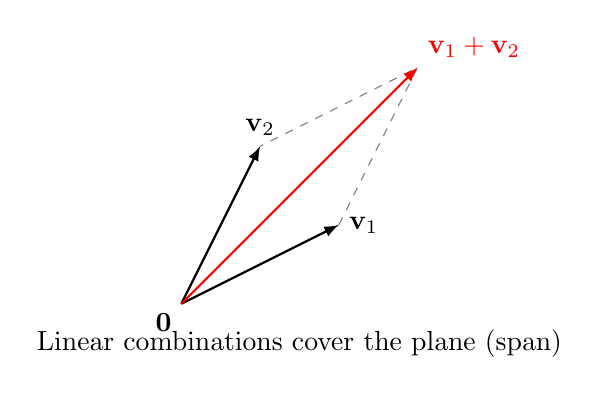
\begin{tikzpicture}[scale=1]
    \coordinate (O) at (0,0);
    \draw[->, thick, -latex] (O) -- (2,1) node[right] {$\mathbf{v}_1$};
    \draw[->, thick, -latex] (O) -- (1,2) node[above] {$\mathbf{v}_2$};
    \draw[dashed, gray] (2,1) -- (3,3) -- (1,2);
    \draw[->, thick, -latex, red] (O) -- (3,3) node[above right] {$\mathbf{v}_1 + \mathbf{v}_2$};
    \node at (O) [below left] {$\mathbf{0}$};
    \node at (1.5, -0.5) {Linear combinations cover the plane (span)};
  \end{tikzpicture}
\end{center}

\begin{definition}[Linear independence]
  A family of vectors $(\mathbf{v}_1,\dots,\mathbf{v}_n)$ in a vector space $V$ is
  \emph{linearly independent} if
  \begin{equation}
    \alpha_1\mathbf{v}_1 + \dots + \alpha_n\mathbf{v}_n = \mathbf{0}
    \quad \text{implies} \quad
    \alpha_1 = \dots = \alpha_n = 0.
  \end{equation}
\end{definition}

\begin{definition}[Basis]
  A \emph{basis} of a vector space $V$ is a linearly independent set of vectors that spans $V$.
  That is, a family $\mathcal{B} = (\mathbf{v}_1,\dots,\mathbf{v}_n)$ is a basis if:
  \begin{enumerate}
    \item $\mathcal{B}$ is linearly independent, and
    \item every vector $\mathbf{v} \in V$ can be written as a linear combination
          $\mathbf{v} = \alpha_1\mathbf{v}_1 + \dots + \alpha_n\mathbf{v}_n$ for some scalars $\alpha_1,\dots,\alpha_n$.
  \end{enumerate}
\end{definition}

\begin{definition}[Dimension]
  The \emph{dimension} of a vector space $V$, denoted $\dim(V)$, is the number of vectors in any basis of $V$.
  If $V$ has a finite basis, then $V$ is \emph{finite-dimensional}; otherwise, $V$ is \emph{infinite-dimensional}.
\end{definition}

\section{Inner Product Spaces}

\begin{definition}[Inner product space]
  An \emph{inner product space} is a vector space $V$ over $\mathbb{F}$ (where $\mathbb{F} = \mathbb{R}$ or $\mathbb{C}$)
  equipped with an inner product $\langle \cdot, \cdot \rangle : V \times V \to \mathbb{F}$ satisfying:
  \begin{enumerate}
    \item Conjugate symmetry: $\langle \mathbf{v}, \mathbf{w} \rangle = \overline{\langle \mathbf{w}, \mathbf{v} \rangle}$,
    \item Linearity in the first argument: $\langle \alpha\mathbf{u} + \beta\mathbf{v}, \mathbf{w} \rangle = \alpha\langle \mathbf{u}, \mathbf{w} \rangle + \beta\langle \mathbf{v}, \mathbf{w} \rangle$,
    \item Positive definiteness: $\langle \mathbf{v}, \mathbf{v} \rangle \geq 0$ with equality if and only if $\mathbf{v} = \mathbf{0}$.
  \end{enumerate}
\end{definition}

\begin{definition}[Orthogonality]
  Two vectors $\mathbf{v}, \mathbf{w} \in V$ are \emph{orthogonal} if $\langle \mathbf{v}, \mathbf{w} \rangle = 0$.
  A set of vectors $\{\mathbf{v}_1,\dots,\mathbf{v}_n\}$ is \emph{orthogonal} if the vectors are pairwise orthogonal.
  An orthogonal set is \emph{orthonormal} if additionally $\langle \mathbf{v}_i, \mathbf{v}_i \rangle = 1$ for all $i$.
\end{definition}

\begin{definition}[Frobenius inner product for matrices]
  The space of $m \times n$ matrices $\mathbb{R}^{m \times n}$ (or $\mathbb{C}^{m \times n}$) is an inner product space with the \emph{Frobenius inner product}
  \begin{equation}
    \langle \mathbf{A}, \mathbf{B} \rangle_F = \operatorname{tr}(\mathbf{A}^{\mathsf{T}}\mathbf{B}) = \sum_{i=1}^{m}\sum_{j=1}^{n} a_{ij}b_{ij}.
  \end{equation}
\end{definition}

\begin{definition}[Frobenius norm]
  The \emph{Frobenius norm} of a matrix $\mathbf{A} \in \mathbb{R}^{m \times n}$ is
  \begin{equation}
    \|\mathbf{A}\|_F = \sqrt{\sum_{i=1}^{m}\sum_{j=1}^{n} a_{ij}^2} = \sqrt{\langle \mathbf{A}, \mathbf{A} \rangle_F}.
  \end{equation}
\end{definition}

\begin{proposition}[Frobenius norm via trace]\label{prop:frobenius-trace}
  For any matrix $\mathbf{A} \in \mathbb{R}^{m \times n}$,
  \begin{equation}\label{eq:frobenius-trace}
    \|\mathbf{A}\|_F^2 = \operatorname{tr}(\mathbf{A}^{\mathsf{T}}\mathbf{A}) = \operatorname{tr}(\mathbf{A}\mathbf{A}^{\mathsf{T}}).
  \end{equation}
\end{proposition}

\begin{proof}
  Let $\mathbf{A} = (a_{ij}) \in \mathbb{R}^{m \times n}$. We compute $\mathbf{A}^{\mathsf{T}}\mathbf{A} \in \mathbb{R}^{n \times n}$:
  \[
    (\mathbf{A}^{\mathsf{T}}\mathbf{A})_{jk} = \sum_{i=1}^{m} a_{ij} a_{ik}.
  \]
  The diagonal entries are:
  \[
    (\mathbf{A}^{\mathsf{T}}\mathbf{A})_{jj} = \sum_{i=1}^{m} a_{ij}^2.
  \]
  Taking the trace (sum of diagonal entries):
  \[
    \operatorname{tr}(\mathbf{A}^{\mathsf{T}}\mathbf{A}) = \sum_{j=1}^{n} (\mathbf{A}^{\mathsf{T}}\mathbf{A})_{jj} = \sum_{j=1}^{n} \sum_{i=1}^{m} a_{ij}^2 = \sum_{i=1}^{m}\sum_{j=1}^{n} a_{ij}^2 = \|\mathbf{A}\|_F^2.
  \]

  For the second equality, compute $\mathbf{A}\mathbf{A}^{\mathsf{T}} \in \mathbb{R}^{m \times m}$:
  \[
    (\mathbf{A}\mathbf{A}^{\mathsf{T}})_{ik} = \sum_{j=1}^{n} a_{ij} a_{kj}.
  \]
  The diagonal entries are:
  \[
    (\mathbf{A}\mathbf{A}^{\mathsf{T}})_{ii} = \sum_{j=1}^{n} a_{ij}^2.
  \]
  Taking the trace:
  \[
    \operatorname{tr}(\mathbf{A}\mathbf{A}^{\mathsf{T}}) = \sum_{i=1}^{m} (\mathbf{A}\mathbf{A}^{\mathsf{T}})_{ii} = \sum_{i=1}^{m} \sum_{j=1}^{n} a_{ij}^2 = \|\mathbf{A}\|_F^2.
  \]
\end{proof}

\begin{remark}
  The Frobenius norm treats a matrix as a vector by summing the squares of all entries.
  For a matrix with rows $\mathbf{a}_1^{\mathsf{T}},\dots,\mathbf{a}_m^{\mathsf{T}} \in \mathbb{R}^n$, we have
  \[
    \|\mathbf{A}\|_F^2 = \sum_{i=1}^{m} \|\mathbf{a}_i\|^2.
  \]
  The Frobenius norm is submultiplicative: $\|\mathbf{A}\mathbf{B}\|_F \leq \|\mathbf{A}\|_F \|\mathbf{B}\|_F$.
\end{remark}

\begin{theorem}[Gram--Schmidt decomposition]
  Let $V$ be an inner product space and let $(\mathbf{v}_1,\dots,\mathbf{v}_n)$ be a linearly independent family of vectors in $V$.
  Then there exists an orthonormal family $(\mathbf{u}_1,\dots,\mathbf{u}_n)$ such that for each $k = 1,\dots,n$,
  \[
    \operatorname{span}(\mathbf{v}_1,\dots,\mathbf{v}_k) = \operatorname{span}(\mathbf{u}_1,\dots,\mathbf{u}_k).
  \]
  Moreover, the vectors $\mathbf{u}_k$ can be constructed recursively by the Gram--Schmidt process:
  \begin{align}
    \mathbf{w}_1 & = \mathbf{v}_1, \quad \mathbf{u}_1 = \frac{\mathbf{w}_1}{\|\mathbf{w}_1\|}, \label{eq:gs-base}                                                                           \\
    \mathbf{w}_k & = \mathbf{v}_k - \sum_{j=1}^{k-1} \langle \mathbf{v}_k, \mathbf{u}_j \rangle \mathbf{u}_j, \quad \mathbf{u}_k = \frac{\mathbf{w}_k}{\|\mathbf{w}_k\|} \label{eq:gs-step}
  \end{align}
  for $k = 2,\dots,n$, where $\|\mathbf{v}\| = \sqrt{\langle \mathbf{v}, \mathbf{v} \rangle}$.
\end{theorem}

\begin{proof}
  We proceed by induction on $k$. For the base case $k=1$, set $\mathbf{u}_1 = \mathbf{v}_1 / \|\mathbf{v}_1\|$.
  Since $\mathbf{v}_1 \neq \mathbf{0}$ (by linear independence), we have $\|\mathbf{u}_1\| = 1$,
  and clearly $\operatorname{span}(\mathbf{v}_1) = \operatorname{span}(\mathbf{u}_1)$.

  Now assume we have constructed orthonormal vectors $\mathbf{u}_1,\dots,\mathbf{u}_{k-1}$ such that
  $\operatorname{span}(\mathbf{v}_1,\dots,\mathbf{v}_j) = \operatorname{span}(\mathbf{u}_1,\dots,\mathbf{u}_j)$ for all $j < k$.

  Define
  \[
    \mathbf{w}_k = \mathbf{v}_k - \sum_{j=1}^{k-1} \langle \mathbf{v}_k, \mathbf{u}_j \rangle \mathbf{u}_j.
  \]
  We claim that $\mathbf{w}_k \neq \mathbf{0}$ and that $\mathbf{w}_k$ is orthogonal to each $\mathbf{u}_i$ for $i < k$.

  To see orthogonality, for any $1 \leq i \leq k-1$, we compute:
  \begin{align*}
    \langle \mathbf{w}_k, \mathbf{u}_i \rangle
     & = \left\langle \mathbf{v}_k - \sum_{j=1}^{k-1} \langle \mathbf{v}_k, \mathbf{u}_j \rangle \mathbf{u}_j, \mathbf{u}_i \right\rangle                    \\
     & = \langle \mathbf{v}_k, \mathbf{u}_i \rangle - \sum_{j=1}^{k-1} \langle \mathbf{v}_k, \mathbf{u}_j \rangle \langle \mathbf{u}_j, \mathbf{u}_i \rangle \\
     & = \langle \mathbf{v}_k, \mathbf{u}_i \rangle - \langle \mathbf{v}_k, \mathbf{u}_i \rangle = 0,
  \end{align*}
  where we used orthonormality: $\langle \mathbf{u}_j, \mathbf{u}_i \rangle = \delta_{ij}$.

  To see that $\mathbf{w}_k \neq \mathbf{0}$, suppose $\mathbf{w}_k = \mathbf{0}$. Then
  \[
    \mathbf{v}_k = \sum_{j=1}^{k-1} \langle \mathbf{v}_k, \mathbf{u}_j \rangle \mathbf{u}_j \in \operatorname{span}(\mathbf{u}_1,\dots,\mathbf{u}_{k-1}) = \operatorname{span}(\mathbf{v}_1,\dots,\mathbf{v}_{k-1}),
  \]
  contradicting the linear independence of $(\mathbf{v}_1,\dots,\mathbf{v}_n)$.

  Thus we can set $\mathbf{u}_k = \mathbf{w}_k / \|\mathbf{w}_k\|$, which has norm $1$ and is orthogonal to $\mathbf{u}_1,\dots,\mathbf{u}_{k-1}$.
  By construction, $\mathbf{v}_k \in \operatorname{span}(\mathbf{u}_1,\dots,\mathbf{u}_k)$ and $\mathbf{u}_k \in \operatorname{span}(\mathbf{v}_1,\dots,\mathbf{v}_k)$,
  so $\operatorname{span}(\mathbf{v}_1,\dots,\mathbf{v}_k) = \operatorname{span}(\mathbf{u}_1,\dots,\mathbf{u}_k)$.
\end{proof}

\begin{remark}[Applications of Gram--Schmidt]
  The Gram--Schmidt process is fundamental across many fields:
  \begin{itemize}
    \item \textbf{Machine learning}: QR decomposition (based on Gram--Schmidt) is used for numerically stable least-squares regression. Orthogonalizing feature vectors removes redundancy and improves conditioning of optimization problems.

    \item \textbf{Quantum mechanics}: States in a quantum system must be represented by orthonormal vectors in a Hilbert space. Gram--Schmidt is used to orthogonalize measurement bases and construct complete orthonormal sets of wavefunctions.

    \item \textbf{Signal processing}: Constructing orthonormal bases (like wavelets or Fourier bases) for signal decomposition. Orthogonal projections onto signal subspaces are used in noise reduction and compression.

    \item \textbf{Numerical analysis}: The QR algorithm for eigenvalue computation relies on repeated Gram--Schmidt orthogonalization. Stable numerical solvers for differential equations use orthogonal polynomial bases constructed via Gram--Schmidt.
  \end{itemize}
\end{remark}

\section{Linear Maps}

\begin{definition}[Linear map]
  Let $V$ and $W$ be vector spaces over a field $\mathbb{F}$.
  A map $T : V \to W$ is a \emph{linear map} (or \emph{linear transformation}) if for all $\mathbf{v}_1, \mathbf{v}_2 \in V$ and $\alpha, \beta \in \mathbb{F}$,
  \begin{equation}
    T(\alpha\mathbf{v}_1 + \beta\mathbf{v}_2) = \alpha T(\mathbf{v}_1) + \beta T(\mathbf{v}_2).
  \end{equation}
  A linear map from a vector space to itself, $T : V \to V$, is called a \emph{linear operator}.
\end{definition}

\begin{definition}[Image and kernel]
  Let $T : V \to W$ be a linear map. The \emph{image} (or \emph{range}) of $T$ is
  \begin{equation}
    \operatorname{im}(T) = \{T(\mathbf{v}) : \mathbf{v} \in V\} \subseteq W.
  \end{equation}
  The \emph{kernel} (or \emph{null space}) of $T$ is
  \begin{equation}
    \ker(T) = \{\mathbf{v} \in V : T(\mathbf{v}) = \mathbf{0}\} \subseteq V.
  \end{equation}
\end{definition}

\section{Matrix Representations}

\subsection{Motivation}

Linear maps between abstract vector spaces (like function spaces or polynomial spaces) seem very different from
matrix-vector multiplication. However, once we choose bases, every linear map can be represented as a matrix.
This is the bridge between abstract linear algebra and concrete computation.

\textbf{The key insight}: A basis gives us a "coordinate system" that identifies an abstract vector space $V$ with $\mathbb{F}^n$.
Once we have coordinates, linear maps become matrices.

Throughout this section, let $V$ and $W$ be finite-dimensional vector spaces over $\mathbb{F}$,
with $\dim(V) = n$ and $\dim(W) = m$.

\begin{definition}[Coordinate isomorphism]
  Let $V$ be a vector space with basis $\mathcal{B} = (\mathbf{v}_1,\dots,\mathbf{v}_n)$.
  The \emph{coordinate map} (or \emph{coordinate isomorphism}) is the map $\Phi_{\mathcal{B}} : V \to \mathbb{F}^n$ defined by
  \begin{equation}
    \Phi_{\mathcal{B}}\left(\sum_{i=1}^{n} x_i \mathbf{v}_i\right) = \begin{pmatrix} x_1 \\ \vdots \\ x_n \end{pmatrix}.
  \end{equation}
  This map is a linear isomorphism: it is bijective and preserves the vector space structure.
\end{definition}

\begin{remark}
  The coordinate map $\Phi_{\mathcal{B}}$ identifies abstract vectors in $V$ with concrete column vectors in $\mathbb{F}^n$.
  It is an isomorphism because:
  \begin{itemize}
    \item Every vector $\mathbf{v} \in V$ has a unique representation as a linear combination of basis vectors.
    \item The map preserves addition and scalar multiplication.
  \end{itemize}
\end{remark}

\begin{theorem}[Fundamental theorem: Every linear map is a matrix]\label{thm:fundamental-linalg}
  Let $T : V \to W$ be a linear map between finite-dimensional vector spaces.
  Fix bases $\mathcal{B}_V = (\mathbf{v}_1,\dots,\mathbf{v}_n)$ of $V$ and $\mathcal{B}_W = (\mathbf{w}_1,\dots,\mathbf{w}_m)$ of $W$,
  and let $\Phi_V : V \to \mathbb{F}^n$ and $\Phi_W : W \to \mathbb{F}^m$ be the coordinate isomorphisms.

  Then there exists a unique matrix $\mathbf{A} \in \mathbb{F}^{m \times n}$ such that
  \begin{equation}\label{eq:matrix-formula}
    \mathbf{A} = \Phi_W \circ T \circ \Phi_V^{-1}.
  \end{equation}
  Equivalently, the following diagram commutes:
  \[
    \begin{tikzcd}[row sep=2.5cm, column sep=2.5cm]
      V \arrow[r, "T"] \arrow[d, swap, "\Phi_V" {yshift=2pt}]
      & W \arrow[d, "\Phi_W" {yshift=2pt}] \\
      \mathbb{F}^n \arrow[r, swap, "\mathbf{A}"]
      & \mathbb{F}^m
    \end{tikzcd}
  \]

  \textbf{How to construct $\mathbf{A}$}: Apply $T$ to each basis vector $\mathbf{v}_j$ and write the result in the basis $\mathcal{B}_W$:
  \begin{equation}\label{eq:matrix-columns}
    T(\mathbf{v}_j) = \sum_{i=1}^{m} a_{ij} \mathbf{w}_i.
  \end{equation}
  Then the $j$-th column of $\mathbf{A}$ is $(a_{1j}, a_{2j}, \dots, a_{mj})^{\mathsf{T}}$.
\end{theorem}

\begin{proof}
  Define the matrix $\mathbf{A} = (a_{ij}) \in \mathbb{F}^{m \times n}$ using the coefficients from \eqref{eq:matrix-columns}.
  We must show that the diagram commutes, i.e., that $\Phi_W \circ T = \mathbf{A} \circ \Phi_V$.

  Let $\mathbf{v} = \sum_{j=1}^{n} x_j \mathbf{v}_j \in V$ be arbitrary. Then $\Phi_V(\mathbf{v}) = (x_1, \dots, x_n)^{\mathsf{T}}$.

  \textbf{Top path} ($V \to W \to \mathbb{F}^m$): Apply $T$ then $\Phi_W$.
  \begin{align*}
    T(\mathbf{v}) & = T\left(\sum_{j=1}^{n} x_j \mathbf{v}_j\right) = \sum_{j=1}^{n} x_j T(\mathbf{v}_j) \quad \text{(by linearity)}              \\
                  & = \sum_{j=1}^{n} x_j \sum_{i=1}^{m} a_{ij} \mathbf{w}_i = \sum_{i=1}^{m} \left(\sum_{j=1}^{n} a_{ij} x_j\right) \mathbf{w}_i.
  \end{align*}
  Applying $\Phi_W$ gives
  \[
    \Phi_W(T(\mathbf{v})) = \begin{pmatrix} \sum_{j=1}^{n} a_{1j} x_j \\ \vdots \\ \sum_{j=1}^{n} a_{mj} x_j \end{pmatrix}.
  \]

  \textbf{Bottom path} ($V \to \mathbb{F}^n \to \mathbb{F}^m$): Apply $\Phi_V$ then $\mathbf{A}$.
  \[
    \mathbf{A} \, \Phi_V(\mathbf{v}) = \mathbf{A} \begin{pmatrix} x_1 \\ \vdots \\ x_n \end{pmatrix} = \begin{pmatrix} \sum_{j=1}^{n} a_{1j} x_j \\ \vdots \\ \sum_{j=1}^{n} a_{mj} x_j \end{pmatrix}.
  \]

  Both paths give the same result, so the diagram commutes.

  Uniqueness: The matrix $\mathbf{A}$ is uniquely determined by requiring commutativity at the basis vectors $\mathbf{v}_j$,
  which forces the columns to be as in \eqref{eq:matrix-columns}. By linearity, this determines $\mathbf{A}$ on all of $V$.
\end{proof}

\begin{remark}[Significance of the formula $\mathbf{A} = \Phi_W \circ T \circ \Phi_V^{-1}$]
  The formula \eqref{eq:matrix-formula} reveals the deep connection between abstract linear maps and matrices:
  \begin{itemize}
    \item \textbf{To compute $\mathbf{A}\mathbf{x}$}: Start with coordinates $\mathbf{x} \in \mathbb{F}^n$, convert to abstract vector via $\Phi_V^{-1}$,
          apply the abstract map $T$, then convert back to coordinates via $\Phi_W$.

    \item \textbf{The coordinate maps are isomorphisms}: Both $\Phi_V$ and $\Phi_W$ are linear, bijective, and invertible.
          This means every finite-dimensional vector space is "the same as" $\mathbb{F}^n$ once we pick a basis.

    \item \textbf{Change of perspective}: The same linear transformation $T$ has different matrix representations depending on
          the choice of bases. The matrix $\mathbf{A}$ is not intrinsic to $T$, but depends on our coordinate systems.

    \item \textbf{Composition of maps}: The formula shows that matrix multiplication corresponds to composition of linear maps
          after translating between abstract and coordinate viewpoints.
  \end{itemize}
\end{remark}

\begin{remark}[Applications: Why every linear map is a matrix]
  This fundamental theorem bridges abstract mathematics and computation:
  \begin{itemize}
    \item \textbf{Machine learning}: Neural network layers are linear transformations between high-dimensional feature spaces. The theorem guarantees that choosing a basis (e.g., pixel coordinates, word embeddings) allows us to represent these transformations as matrix multiplications, enabling GPU-accelerated training.

    \item \textbf{Computer graphics}: Transformations like rotations, scaling, and projections act on infinite-dimensional function spaces (continuous surfaces). By discretizing to vertices and choosing a basis, the theorem shows these become finite matrix operations that GPUs can execute in real-time.

    \item \textbf{Quantum computing}: Quantum gates are unitary operators on infinite-dimensional Hilbert spaces. The theorem ensures that restricting to finite-dimensional qubit spaces gives matrix representations, making quantum circuits implementable on physical hardware.

    \item \textbf{Differential equations}: Linear differential operators (like $\frac{d}{dx}$) act on infinite-dimensional function spaces. Choosing a basis (Fourier modes, finite elements) converts them to matrices, enabling numerical solution methods.

    \item \textbf{Theoretical physics}: Symmetries of physical systems are represented by abstract group actions. The theorem shows that these symmetries have matrix representations, connecting abstract symmetry principles to concrete calculations in quantum field theory and particle physics.
  \end{itemize}
  \textbf{Key insight}: The theorem shows that \emph{choosing coordinates is the bridge between abstract theory and practical computation}. Different bases give different matrix representations, but all encode the same underlying linear transformation.
\end{remark}



\begin{remark}
  We sometimes write $[T]_{\mathcal{B}_W,\mathcal{B}_V} = \mathbf{A}$ to denote the matrix representation of $T$ with respect to the given bases.
  When $V = W$ and both bases are the same $\mathcal{B}$, we write $[T]_{\mathcal{B}}$.
\end{remark}

\begin{corollary}[The case of $\mathbb{F}^n$]
  When working in $\mathbb{F}^n$ with the standard basis $\mathcal{E} = (\mathbf{e}_1,\dots,\mathbf{e}_n)$,
  the coordinate map is the identity ($\Phi_{\mathcal{E}}(\mathbf{x}) = \mathbf{x}$).
  Therefore, for any linear map $T : \mathbb{F}^n \to \mathbb{F}^m$,
  \begin{equation}
    T(\mathbf{x}) = \mathbf{A}\mathbf{x},
  \end{equation}
  where $\mathbf{A} \in \mathbb{F}^{m \times n}$ has $j$-th column $\mathbf{A}_{:,j} = T(\mathbf{e}_j)$.
  In this case, the linear map $T$ and its matrix $\mathbf{A}$ are identified.
\end{corollary}

\subsection{Subspaces of $\mathbb{R}^d$}

For the special case of $\mathbb{R}^d$ with the standard inner product $\langle \mathbf{x}, \mathbf{y} \rangle = \mathbf{x}^{\mathsf{T}}\mathbf{y}$,
we have the following useful characterization.

\begin{lemma}[Orthonormal matrix characterization of subspaces]
  Let $S \subseteq \mathbb{R}^d$ be a $k$-dimensional subspace. Then:
  \begin{enumerate}
    \item There exists a matrix $\mathbf{W} \in \mathbb{R}^{d \times k}$ such that the columns of $\mathbf{W}$ form an orthonormal basis of $S$.
    \item Conversely, any matrix $\mathbf{W} \in \mathbb{R}^{d \times k}$ with
          \begin{equation}
            \mathbf{W}^{\mathsf{T}}\mathbf{W} = \mathbf{I}_k
          \end{equation}
          defines a $k$-dimensional subspace
          \begin{equation}
            S = \{\mathbf{W}\mathbf{z} : \mathbf{z} \in \mathbb{R}^k\}.
          \end{equation}
  \end{enumerate}
\end{lemma}

\begin{proof}
  (1) Since $S$ is a $k$-dimensional subspace of $\mathbb{R}^d$, it has a basis $(\mathbf{v}_1,\dots,\mathbf{v}_k)$.
  By the Gram--Schmidt decomposition, we can construct an orthonormal basis $(\mathbf{u}_1,\dots,\mathbf{u}_k)$ for $S$.
  Let $\mathbf{W} \in \mathbb{R}^{d \times k}$ be the matrix whose columns are $\mathbf{u}_1,\dots,\mathbf{u}_k$.
  Then the columns of $\mathbf{W}$ form an orthonormal basis of $S$.

  (2) Suppose $\mathbf{W} \in \mathbb{R}^{d \times k}$ satisfies $\mathbf{W}^{\mathsf{T}}\mathbf{W} = \mathbf{I}_k$.
  This condition means that the columns $\mathbf{w}_1,\dots,\mathbf{w}_k$ of $\mathbf{W}$ are orthonormal:
  $\langle \mathbf{w}_i, \mathbf{w}_j \rangle = \delta_{ij}$ for all $i,j$.
  In particular, the columns are linearly independent, so $S = \operatorname{span}(\mathbf{w}_1,\dots,\mathbf{w}_k) = \{\mathbf{W}\mathbf{z} : \mathbf{z} \in \mathbb{R}^k\}$
  is a $k$-dimensional subspace of $\mathbb{R}^d$.
\end{proof}

\section{Eigenvalues and Eigenvectors}

\begin{definition}[Eigenvalue and eigenvector]
  Let $T : V \to V$ be a linear operator on a vector space $V$ over $\mathbb{F}$.
  A scalar $\lambda \in \mathbb{F}$ is an \emph{eigenvalue} of $T$ if there exists a nonzero vector $\mathbf{v} \in V$ such that
  \begin{equation}
    T(\mathbf{v}) = \lambda \mathbf{v}.
  \end{equation}
  The vector $\mathbf{v}$ is called an \emph{eigenvector} corresponding to $\lambda$.
\end{definition}

\begin{remark}
  For matrices $\mathbf{A} \in \mathbb{F}^{n \times n}$, the eigenvalue equation becomes $\mathbf{A}\mathbf{v} = \lambda \mathbf{v}$.
  Equivalently, $(\mathbf{A} - \lambda \mathbf{I})\mathbf{v} = \mathbf{0}$, so $\lambda$ is an eigenvalue if and only if
  $\det(\mathbf{A} - \lambda \mathbf{I}) = 0$.
\end{remark}

\begin{definition}[Symmetric matrix]
  A matrix $\mathbf{A} \in \mathbb{R}^{n \times n}$ is \emph{symmetric} if $\mathbf{A}^{\mathsf{T}} = \mathbf{A}$.
\end{definition}

\begin{definition}[Definiteness of symmetric matrices]\label{def:definiteness}
  Let $\mathbf{A} \in \mathbb{R}^{n \times n}$ be a symmetric matrix. We classify $\mathbf{A}$ based on the sign of the quadratic form $\mathbf{x}^{\mathsf{T}}\mathbf{A}\mathbf{x}$:
  \begin{enumerate}
    \item $\mathbf{A}$ is \emph{positive definite} if $\mathbf{x}^{\mathsf{T}}\mathbf{A}\mathbf{x} > 0$ for all $\mathbf{x} \neq \mathbf{0}$.
    \item $\mathbf{A}$ is \emph{positive semidefinite} if $\mathbf{x}^{\mathsf{T}}\mathbf{A}\mathbf{x} \geq 0$ for all $\mathbf{x} \in \mathbb{R}^n$.
    \item $\mathbf{A}$ is \emph{negative definite} if $\mathbf{x}^{\mathsf{T}}\mathbf{A}\mathbf{x} < 0$ for all $\mathbf{x} \neq \mathbf{0}$.
    \item $\mathbf{A}$ is \emph{negative semidefinite} if $\mathbf{x}^{\mathsf{T}}\mathbf{A}\mathbf{x} \leq 0$ for all $\mathbf{x} \in \mathbb{R}^n$.
    \item $\mathbf{A}$ is \emph{indefinite} if $\mathbf{x}^{\mathsf{T}}\mathbf{A}\mathbf{x}$ takes both positive and negative values.
  \end{enumerate}
\end{definition}

\begin{remark}
  For a symmetric matrix $\mathbf{A}$ with eigenvalues $\lambda_1,\dots,\lambda_n$:
  \begin{itemize}
    \item $\mathbf{A}$ is positive definite $\Leftrightarrow$ all $\lambda_i > 0$.
    \item $\mathbf{A}$ is positive semidefinite $\Leftrightarrow$ all $\lambda_i \geq 0$.
    \item $\mathbf{A}$ is negative definite $\Leftrightarrow$ all $\lambda_i < 0$.
    \item $\mathbf{A}$ is negative semidefinite $\Leftrightarrow$ all $\lambda_i \leq 0$.
    \item $\mathbf{A}$ is indefinite $\Leftrightarrow$ $\mathbf{A}$ has both positive and negative eigenvalues.
  \end{itemize}
  This characterization follows from the spectral theorem: if $\mathbf{A} = \mathbf{U}\mathbf{\Lambda}\mathbf{U}^{\mathsf{T}}$ with $\mathbf{U}$ orthogonal, then
  \[
    \mathbf{x}^{\mathsf{T}}\mathbf{A}\mathbf{x} = \mathbf{x}^{\mathsf{T}}\mathbf{U}\mathbf{\Lambda}\mathbf{U}^{\mathsf{T}}\mathbf{x} = \sum_{i=1}^{n} \lambda_i (\mathbf{u}_i^{\mathsf{T}}\mathbf{x})^2,
  \]
  where $\mathbf{u}_i$ are the columns of $\mathbf{U}$.
\end{remark}

\begin{lemma}[Eigenvalues of symmetric matrices are real]\label{lem:symmetric-real-eigenvalues}
  Let $\mathbf{A} \in \mathbb{R}^{n \times n}$ be symmetric. Then all eigenvalues of $\mathbf{A}$ are real,
  and we can choose corresponding eigenvectors to be real.
\end{lemma}

\begin{proof}
  Let $\lambda$ be an eigenvalue with eigenvector $\mathbf{v} \in \mathbb{C}^n$ (allowing complex vectors).
  Then $\mathbf{A}\mathbf{v} = \lambda \mathbf{v}$ with $\mathbf{v} \neq \mathbf{0}$.

  Taking the conjugate transpose of both sides: $\overline{\mathbf{v}}^{\mathsf{T}} \mathbf{A}^{\mathsf{T}} = \overline{\lambda} \overline{\mathbf{v}}^{\mathsf{T}}$.
  Since $\mathbf{A}$ is real and symmetric, $\mathbf{A}^{\mathsf{T}} = \mathbf{A}$, so $\overline{\mathbf{v}}^{\mathsf{T}} \mathbf{A} = \overline{\lambda} \overline{\mathbf{v}}^{\mathsf{T}}$.

  Now multiply the original equation on the left by $\overline{\mathbf{v}}^{\mathsf{T}}$:
  \[
    \overline{\mathbf{v}}^{\mathsf{T}} \mathbf{A} \mathbf{v} = \lambda \overline{\mathbf{v}}^{\mathsf{T}} \mathbf{v}.
  \]
  And multiply the conjugated equation on the right by $\mathbf{v}$:
  \[
    \overline{\mathbf{v}}^{\mathsf{T}} \mathbf{A} \mathbf{v} = \overline{\lambda} \overline{\mathbf{v}}^{\mathsf{T}} \mathbf{v}.
  \]
  Since both equal $\overline{\mathbf{v}}^{\mathsf{T}} \mathbf{A} \mathbf{v}$ and $\overline{\mathbf{v}}^{\mathsf{T}} \mathbf{v} = \|\mathbf{v}\|^2 > 0$,
  we have $\lambda = \overline{\lambda}$, so $\lambda \in \mathbb{R}$.

  For a real eigenvalue, we can find a real eigenvector by taking the real or imaginary part of a complex eigenvector.
\end{proof}

\begin{lemma}[Eigenvectors for distinct eigenvalues are orthogonal]\label{lem:distinct-eigenvalues-orthogonal}
  Let $\mathbf{A} \in \mathbb{R}^{n \times n}$ be symmetric. If $\mathbf{v}_1, \mathbf{v}_2$ are eigenvectors with distinct eigenvalues
  $\lambda_1 \neq \lambda_2$, then $\mathbf{v}_1 \perp \mathbf{v}_2$.
\end{lemma}

\begin{proof}
  We have $\mathbf{A}\mathbf{v}_1 = \lambda_1 \mathbf{v}_1$ and $\mathbf{A}\mathbf{v}_2 = \lambda_2 \mathbf{v}_2$. Then
  \begin{align*}
    \lambda_1 \langle \mathbf{v}_1, \mathbf{v}_2 \rangle
     & = \langle \lambda_1 \mathbf{v}_1, \mathbf{v}_2 \rangle = \langle \mathbf{A}\mathbf{v}_1, \mathbf{v}_2 \rangle                                                       \\
     & = \mathbf{v}_1^{\mathsf{T}} \mathbf{A}^{\mathsf{T}} \mathbf{v}_2 = \mathbf{v}_1^{\mathsf{T}} \mathbf{A} \mathbf{v}_2 \quad \text{(since $\mathbf{A}$ is symmetric)} \\
     & = \mathbf{v}_1^{\mathsf{T}} (\lambda_2 \mathbf{v}_2) = \lambda_2 \langle \mathbf{v}_1, \mathbf{v}_2 \rangle.
  \end{align*}
  Therefore, $(\lambda_1 - \lambda_2) \langle \mathbf{v}_1, \mathbf{v}_2 \rangle = 0$.
  Since $\lambda_1 \neq \lambda_2$, we must have $\langle \mathbf{v}_1, \mathbf{v}_2 \rangle = 0$.
\end{proof}

\begin{theorem}[Spectral theorem for symmetric matrices]\label{thm:spectral}
  Let $\mathbf{A} \in \mathbb{R}^{n \times n}$ be a symmetric matrix. Then there exists an orthonormal basis of $\mathbb{R}^n$
  consisting of eigenvectors of $\mathbf{A}$. Moreover, we can write
  \begin{equation}
    \mathbf{A} = \mathbf{U}\mathbf{\Lambda}\mathbf{U}^{\mathsf{T}},
  \end{equation}
  where $\mathbf{U} \in \mathbb{R}^{n \times n}$ is orthogonal ($\mathbf{U}^{\mathsf{T}}\mathbf{U} = \mathbf{I}$) with columns being orthonormal eigenvectors,
  and $\mathbf{\Lambda} = \operatorname{diag}(\lambda_1,\dots,\lambda_n)$ contains the corresponding eigenvalues.
\end{theorem}

\begin{proof}
  We proceed by induction on $n$.

  \textbf{Base case} ($n = 1$): Any $1 \times 1$ matrix $\mathbf{A} = [a]$ has eigenvalue $\lambda = a$ with eigenvector $\mathbf{u} = [1]$.

  \textbf{Inductive step}: Assume the result holds for $(n-1) \times (n-1)$ symmetric matrices.
  Let $\mathbf{A} \in \mathbb{R}^{n \times n}$ be symmetric.

  By Lemma~\ref{lem:symmetric-real-eigenvalues}, $\mathbf{A}$ has a real eigenvalue $\lambda_1$ with real eigenvector $\mathbf{v}_1$.
  Normalize to get $\mathbf{u}_1 = \mathbf{v}_1 / \|\mathbf{v}_1\|$ with $\|\mathbf{u}_1\| = 1$.

  Extend $\{\mathbf{u}_1\}$ to an orthonormal basis $\{\mathbf{u}_1, \mathbf{w}_2, \dots, \mathbf{w}_n\}$ of $\mathbb{R}^n$
  (using Gram-Schmidt if necessary). Let $\mathbf{Q} = [\mathbf{u}_1 \mid \mathbf{w}_2 \mid \cdots \mid \mathbf{w}_n]$ be orthogonal.

  Consider $\mathbf{B} = \mathbf{Q}^{\mathsf{T}} \mathbf{A} \mathbf{Q}$. The first column of $\mathbf{A}\mathbf{Q}$ is
  \[
    \mathbf{A}\mathbf{u}_1 = \lambda_1 \mathbf{u}_1.
  \]
  So the first column of $\mathbf{Q}^{\mathsf{T}}\mathbf{A}\mathbf{Q}$ is $\mathbf{Q}^{\mathsf{T}}(\lambda_1 \mathbf{u}_1) = \lambda_1 \mathbf{e}_1$.

  Since $\mathbf{B}$ is symmetric (as $\mathbf{B}^{\mathsf{T}} = (\mathbf{Q}^{\mathsf{T}}\mathbf{A}\mathbf{Q})^{\mathsf{T}} = \mathbf{Q}^{\mathsf{T}}\mathbf{A}^{\mathsf{T}}\mathbf{Q} = \mathbf{Q}^{\mathsf{T}}\mathbf{A}\mathbf{Q} = \mathbf{B}$),
  we have
  \[
    \mathbf{B} = \begin{pmatrix} \lambda_1 & \mathbf{0}^{\mathsf{T}} \\ \mathbf{0} & \mathbf{B}' \end{pmatrix},
  \]
  where $\mathbf{B}' \in \mathbb{R}^{(n-1) \times (n-1)}$ is symmetric.

  By the inductive hypothesis, $\mathbf{B}' = \mathbf{V}\mathbf{\Lambda}'\mathbf{V}^{\mathsf{T}}$ where $\mathbf{V}$ is orthogonal and $\mathbf{\Lambda}'$ is diagonal.

  Let $\widetilde{\mathbf{V}} = \begin{pmatrix} 1 & \mathbf{0}^{\mathsf{T}} \\ \mathbf{0} & \mathbf{V} \end{pmatrix}$. Then $\widetilde{\mathbf{V}}$ is orthogonal and
  \[
    \mathbf{B} = \widetilde{\mathbf{V}} \begin{pmatrix} \lambda_1 & \mathbf{0}^{\mathsf{T}} \\ \mathbf{0} & \mathbf{\Lambda}' \end{pmatrix} \widetilde{\mathbf{V}}^{\mathsf{T}}.
  \]

  Setting $\mathbf{U} = \mathbf{Q}\widetilde{\mathbf{V}}$ (orthogonal) and $\mathbf{\Lambda} = \begin{pmatrix} \lambda_1 & \mathbf{0}^{\mathsf{T}} \\ \mathbf{0} & \mathbf{\Lambda}' \end{pmatrix}$ (diagonal), we get
  \[
    \mathbf{A} = \mathbf{Q} \mathbf{B} \mathbf{Q}^{\mathsf{T}} = \mathbf{Q} \widetilde{\mathbf{V}} \mathbf{\Lambda} \widetilde{\mathbf{V}}^{\mathsf{T}} \mathbf{Q}^{\mathsf{T}} = \mathbf{U} \mathbf{\Lambda} \mathbf{U}^{\mathsf{T}}.
  \]
  The columns of $\mathbf{U}$ form an orthonormal basis of eigenvectors.
\end{proof}

\begin{remark}
  The spectral theorem is specific to symmetric (or more generally, self-adjoint) matrices.
  \begin{itemize}
    \item \textbf{What's general}: Any matrix $\mathbf{A} \in \mathbb{C}^{n \times n}$ has $n$ eigenvalues (counted with multiplicity) and can be diagonalized if and only if it has $n$ linearly independent eigenvectors.
    \item \textbf{What's special for symmetric matrices}: Eigenvalues are real, eigenvectors are orthogonal, and diagonalization via orthogonal matrices is always possible.
  \end{itemize}
\end{remark}

\section{Applications of the Spectral Theorem}

The spectral theorem is not just an abstract result; it is the mathematical engine behind many physical theories and modern algorithms.

\subsection{Machine Learning}

\subsubsection{Covariance Matrices and PCA}
In statistics and machine learning, the relationship between random variables $X_1, \dots, X_n$ is captured by the covariance matrix $\mathbf{\Sigma} = \mathbb{E}[(\mathbf{X} - \boldsymbol{\mu})(\mathbf{X} - \boldsymbol{\mu})^{\mathsf{T}}]$.
Since $\mathbf{\Sigma}_{ij} = \operatorname{Cov}(X_i, X_j) = \operatorname{Cov}(X_j, X_i)$, the matrix is symmetric.
The spectral theorem guarantees $\mathbf{\Sigma} = \mathbf{U}\mathbf{\Lambda}\mathbf{U}^{\mathsf{T}}$, where $\mathbf{U}$ contains the principal directions of variation (eigenvectors) and $\mathbf{\Lambda}$ contains the variances along those directions (eigenvalues).

\begin{center}
  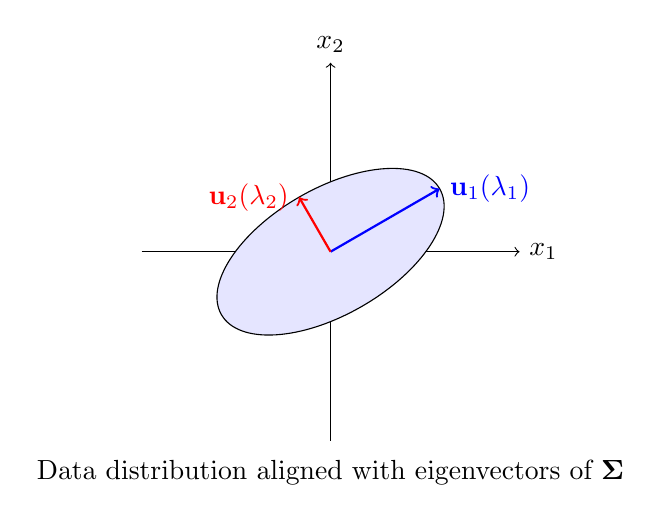
\begin{tikzpicture}[scale=0.8]
    \draw[->] (-3,0) -- (3,0) node[right] {$x_1$};
    \draw[->] (0,-3) -- (0,3) node[above] {$x_2$};
    \draw[rotate=30, fill=blue!10] (0,0) ellipse (2 and 1);
    \draw[->, thick, blue] (0,0) -- (1.73, 1) node[right] {$\mathbf{u}_1 (\lambda_1)$};
    \draw[->, thick, red] (0,0) -- (-0.5, 0.866) node[left] {$\mathbf{u}_2 (\lambda_2)$};
    \node at (0,-3.5) {Data distribution aligned with eigenvectors of $\mathbf{\Sigma}$};
  \end{tikzpicture}
\end{center}

\subsubsection{Kernel Methods (SVMs)}
Kernel methods map data $\mathbf{x} \in \mathcal{X}$ to a high-dimensional feature space $\mathcal{H}$ via $\phi: \mathcal{X} \to \mathcal{H}$. The kernel function is $k(\mathbf{x}, \mathbf{y}) = \langle \phi(\mathbf{x}), \phi(\mathbf{y}) \rangle_{\mathcal{H}}$.
The kernel matrix $\mathbf{K}_{ij} = k(\mathbf{x}_i, \mathbf{x}_j)$ is symmetric and positive semidefinite.
By the spectral theorem, $\mathbf{K} = \mathbf{V}\mathbf{\Lambda}\mathbf{V}^{\mathsf{T}}$ with $\lambda_i \ge 0$. This ensures that $\mathbf{K}$ represents a valid inner product, allowing linear algorithms (like Support Vector Machines) to learn non-linear decision boundaries efficiently.

\subsubsection{Graph Neural Networks}
A graph $G=(V,E)$ is represented by its adjacency matrix $\mathbf{A}$. The Graph Laplacian $\mathbf{L} = \mathbf{D} - \mathbf{A}$ (where $\mathbf{D}$ is the degree matrix) is symmetric.
The spectral decomposition $\mathbf{L} = \mathbf{U}\mathbf{\Lambda}\mathbf{U}^{\mathsf{T}}$ defines the \emph{Graph Fourier Transform}.
For a signal $\mathbf{x} \in \mathbb{R}^{|V|}$ on the nodes, its Fourier transform is $\hat{\mathbf{x}} = \mathbf{U}^{\mathsf{T}}\mathbf{x}$.
Spectral convolutions are defined as $g \star \mathbf{x} = \mathbf{U} g(\mathbf{\Lambda}) \mathbf{U}^{\mathsf{T}} \mathbf{x}$, which is the foundation of spectral Graph Neural Networks (GNNs).

\subsection{Quantum Mechanics}

\subsubsection{Observables as Self-Adjoint Operators}
In quantum mechanics, physical quantities (observables) like position, momentum, and energy are represented by self-adjoint (Hermitian) operators $\hat{A}$ on a Hilbert space $\mathcal{H}$.
The spectral theorem guarantees:
\begin{itemize}
  \item The eigenvalues $a_n$ are real. These are the only possible outcomes of a measurement.
  \item The eigenvectors $|\psi_n\rangle$ form a complete orthonormal basis.
\end{itemize}
Any state $|\psi\rangle$ can be expanded as $|\psi\rangle = \sum_n c_n |\psi_n\rangle$. The probability of measuring $a_n$ is $P(a_n) = |\langle \psi_n | \psi \rangle|^2 = |c_n|^2$.

\subsubsection{Time Evolution}
The dynamics of a quantum system are governed by the Hamiltonian operator $\hat{H}$. The Schrödinger equation is:
\[
  i\hbar \frac{d}{dt}|\psi(t)\rangle = \hat{H}|\psi(t)\rangle.
\]
Using the spectral decomposition $\hat{H} = \sum_n E_n |\psi_n\rangle\langle\psi_n|$, the time evolution operator is:
\[
  e^{-i\hat{H}t/\hbar} = \sum_n e^{-iE_n t/\hbar} |\psi_n\rangle\langle\psi_n|.
\]
This allows us to solve for the state at any time: $|\psi(t)\rangle = \sum_n c_n(0) e^{-iE_n t/\hbar} |\psi_n\rangle$.

\begin{center}
  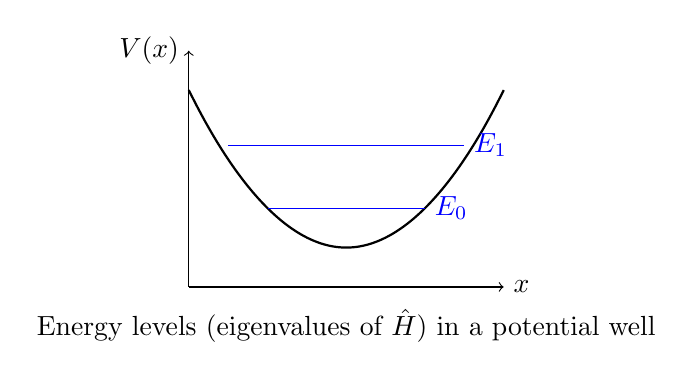
\begin{tikzpicture}
    \draw[->] (0,0) -- (4,0) node[right] {$x$};
    \draw[->] (0,0) -- (0,3) node[left] {$V(x)$};
    \draw[thick] (0,2.5) parabola bend (2,0.5) (4,2.5);
    \draw[blue] (1, 1) -- (3, 1) node[right] {$E_0$};
    \draw[blue] (0.5, 1.8) -- (3.5, 1.8) node[right] {$E_1$};
    \node at (2,-0.5) {Energy levels (eigenvalues of $\hat{H}$) in a potential well};
  \end{tikzpicture}
\end{center}

\subsection{Physics (Classical Mechanics)}

\subsubsection{The Inertia Tensor}
For a rigid body, the angular momentum $\mathbf{L}$ is related to the angular velocity $\boldsymbol{\omega}$ by the inertia tensor $\mathbf{I}$: $\mathbf{L} = \mathbf{I}\boldsymbol{\omega}$.
$\mathbf{I}$ is a symmetric $3 \times 3$ matrix. Its eigenvectors $\mathbf{e}_1, \mathbf{e}_2, \mathbf{e}_3$ define the \emph{principal axes} of rotation.
In this basis, the tensor is diagonal: $\mathbf{I}' = \operatorname{diag}(I_1, I_2, I_3)$.
Rotation about a principal axis is stable (for max/min moments) and simplifies the Euler equations of motion.

\subsubsection{Normal Modes of Vibration}
Coupled oscillators (like masses connected by springs) obey $\mathbf{M}\ddot{\mathbf{x}} + \mathbf{K}\mathbf{x} = \mathbf{0}$, where $\mathbf{M}$ is the mass matrix and $\mathbf{K}$ is the stiffness matrix (both symmetric).
Assuming a solution $\mathbf{x}(t) = \mathbf{v} e^{i\omega t}$, we get the generalized eigenvalue problem:
\[
  (\mathbf{K} - \omega^2 \mathbf{M})\mathbf{v} = \mathbf{0}.
\]
Diagonalizing this system yields the \emph{normal modes} (eigenvectors) where all parts of the system oscillate at the same frequency $\omega \propto \sqrt{\lambda}$.

\subsection{Theoretical Physics}

\subsubsection{Propagators in Quantum Field Theory}
In Quantum Field Theory (QFT), the fundamental object describing particle motion is the \emph{propagator} or Green's function $D(x-y)$. It represents the probability amplitude for a particle to travel from spacetime point $y$ to $x$.

Consider a free scalar field $\phi(x)$ governed by the Klein--Gordon equation:
\[
  (\Box + m^2)\phi(x) = 0, \quad \text{where } \Box = \partial_\mu \partial^\mu = \frac{\partial^2}{\partial t^2} - \nabla^2.
\]
The differential operator $\hat{O} = \Box + m^2$ is translation-invariant, so its "eigenvectors" are the Fourier modes $e^{-ik \cdot x}$ (plane waves) with eigenvalues $-k^2 + m^2$, where $k^2 = (k^0)^2 - |\mathbf{k}|^2$.

The propagator $D(x-y)$ is the inverse of this operator, formally $\hat{O}^{-1}$. Using the spectral decomposition in momentum space (the continuous analog of matrix diagonalization), we write the inverse operator as an integral over the inverse eigenvalues:
\[
  D(x-y) = \int \frac{d^4k}{(2\pi)^4} \frac{e^{-ik \cdot (x-y)}}{m^2 - k^2 - i\epsilon}.
\]
Here, the term $i\epsilon$ is a regularization parameter that shifts the poles of the integrand off the real axis, defining how the contour integral is performed. This choice corresponds to the \emph{Feynman propagator}, which enforces causality: particles propagate forward in time, and antiparticles propagate backward.

\begin{center}
  \begin{tikzpicture}[scale=1.2]
    % Axes
    \draw[->] (-3,0) -- (3,0) node[right] {$\operatorname{Re}(k^0)$};
    \draw[->] (0,-2) -- (0,2) node[above] {$\operatorname{Im}(k^0)$};

    % Poles
    \fill[red] (-1.5, 0.1) circle (2pt) node[above] {$-\omega_k + i\epsilon$};
    \fill[red] (1.5, -0.1) circle (2pt) node[below] {$+\omega_k - i\epsilon$};

    % Contour
    \draw[blue, thick, decoration={markings, mark=at position 0.2 with {\arrow{>}}, mark=at position 0.7 with {\arrow{>}}}, postaction={decorate}] (-2.5,0) -- (-1.8,0) arc (180:360:0.3) -- (1.2,0) arc (180:0:0.3) -- (2.5,0);

    \node at (0, -2.5) {Poles in the complex $k^0$ plane (Feynman contour)};
  \end{tikzpicture}
\end{center}

Physically, this integral implies that a field excitation is a superposition of all possible momentum states, weighted by how close they are to the "mass shell" condition $k^2 = m^2$. The resonance at $k^2 \approx m^2$ dominates macroscopic propagation.

\subsubsection{Stress-Energy Tensor in General Relativity}
The stress-energy tensor $T_{\mu\nu}$ is a symmetric tensor capturing energy and momentum density.
Einstein's equations link geometry to matter: $G_{\mu\nu} = 8\pi G T_{\mu\nu}$.
Because $T_{\mu\nu}$ is symmetric, at any point in spacetime, one can find a local Lorentz frame (eigenbasis) where $T_{\mu\nu}$ is diagonal.
For a perfect fluid, this gives $T_{\mu\nu} = \operatorname{diag}(\rho, p, p, p)$, representing energy density $\rho$ and pressure $p$. This simplifies the study of stars and cosmology.

\section{Singular Value Decomposition}

The spectral theorem applies only to symmetric matrices. The Singular Value Decomposition (SVD) generalizes this to arbitrary rectangular matrices, providing orthogonal diagonalization for any matrix.

\begin{theorem}[Singular Value Decomposition]\label{thm:svd}
  Let $\mathbf{A} \in \mathbb{R}^{m \times n}$ be any matrix with rank $r = \operatorname{rank}(\mathbf{A})$. Then there exist:
  \begin{itemize}
    \item Orthogonal matrix $\mathbf{U} \in \mathbb{R}^{m \times m}$ with $\mathbf{U}^{\mathsf{T}}\mathbf{U} = \mathbf{I}_m$,
    \item Orthogonal matrix $\mathbf{V} \in \mathbb{R}^{n \times n}$ with $\mathbf{V}^{\mathsf{T}}\mathbf{V} = \mathbf{I}_n$,
    \item Diagonal matrix $\mathbf{\Sigma} \in \mathbb{R}^{m \times n}$ with diagonal entries $\sigma_1 \geq \sigma_2 \geq \cdots \geq \sigma_r > 0$ and all other entries zero,
  \end{itemize}
  such that
  \begin{equation}\label{eq:svd}
    \mathbf{A} = \mathbf{U}\mathbf{\Sigma}\mathbf{V}^{\mathsf{T}}.
  \end{equation}
  The values $\sigma_1,\dots,\sigma_r$ are called the \emph{singular values} of $\mathbf{A}$. The columns of $\mathbf{U}$ are the \emph{left singular vectors}, and the columns of $\mathbf{V}$ are the \emph{right singular vectors}.
\end{theorem}

\begin{proof}
  Consider the matrix $\mathbf{A}^{\mathsf{T}}\mathbf{A} \in \mathbb{R}^{n \times n}$. This matrix is symmetric:
  \[
    (\mathbf{A}^{\mathsf{T}}\mathbf{A})^{\mathsf{T}} = \mathbf{A}^{\mathsf{T}}(\mathbf{A}^{\mathsf{T}})^{\mathsf{T}} = \mathbf{A}^{\mathsf{T}}\mathbf{A}.
  \]
  Moreover, it is positive semidefinite: for any $\mathbf{x} \in \mathbb{R}^n$,
  \[
    \mathbf{x}^{\mathsf{T}}(\mathbf{A}^{\mathsf{T}}\mathbf{A})\mathbf{x} = (\mathbf{A}\mathbf{x})^{\mathsf{T}}(\mathbf{A}\mathbf{x}) = \|\mathbf{A}\mathbf{x}\|^2 \geq 0.
  \]

  By the spectral theorem (Theorem~\ref{thm:spectral}), there exists an orthogonal matrix $\mathbf{V} = [\mathbf{v}_1 \mid \cdots \mid \mathbf{v}_n]$ such that
  \[
    \mathbf{A}^{\mathsf{T}}\mathbf{A} = \mathbf{V}\mathbf{\Lambda}\mathbf{V}^{\mathsf{T}},
  \]
  where $\mathbf{\Lambda} = \operatorname{diag}(\lambda_1,\dots,\lambda_n)$ with $\lambda_1 \geq \lambda_2 \geq \cdots \geq \lambda_n \geq 0$.

  Since $\mathbf{A}^{\mathsf{T}}\mathbf{A}$ has rank $r$, exactly $r$ eigenvalues are positive: $\lambda_1,\dots,\lambda_r > 0$ and $\lambda_{r+1} = \cdots = \lambda_n = 0$.

  Define the \emph{singular values} by $\sigma_i = \sqrt{\lambda_i}$ for $i = 1,\dots,r$. Then $\sigma_1 \geq \cdots \geq \sigma_r > 0$.

  \textbf{Constructing the left singular vectors.} For $i = 1,\dots,r$, define
  \[
    \mathbf{u}_i = \frac{1}{\sigma_i} \mathbf{A}\mathbf{v}_i \in \mathbb{R}^m.
  \]
  We verify that $\{\mathbf{u}_1,\dots,\mathbf{u}_r\}$ are orthonormal. For $i, j \leq r$:
  \begin{align*}
    \langle \mathbf{u}_i, \mathbf{u}_j \rangle
     & = \frac{1}{\sigma_i \sigma_j} (\mathbf{A}\mathbf{v}_i)^{\mathsf{T}}(\mathbf{A}\mathbf{v}_j)                                                                                            \\
     & = \frac{1}{\sigma_i \sigma_j} \mathbf{v}_i^{\mathsf{T}} \mathbf{A}^{\mathsf{T}}\mathbf{A} \mathbf{v}_j                                                                                 \\
     & = \frac{1}{\sigma_i \sigma_j} \mathbf{v}_i^{\mathsf{T}} (\lambda_j \mathbf{v}_j)                                                                                                       \\
     & = \frac{\lambda_j}{\sigma_i \sigma_j} \mathbf{v}_i^{\mathsf{T}} \mathbf{v}_j = \frac{\sigma_j^2}{\sigma_i \sigma_j} \delta_{ij} = \frac{\sigma_j}{\sigma_i} \delta_{ij} = \delta_{ij}.
  \end{align*}

  Extend $\{\mathbf{u}_1,\dots,\mathbf{u}_r\}$ to an orthonormal basis $\{\mathbf{u}_1,\dots,\mathbf{u}_m\}$ of $\mathbb{R}^m$ (using Gram-Schmidt if needed). Let $\mathbf{U} = [\mathbf{u}_1 \mid \cdots \mid \mathbf{u}_m]$.

  \textbf{Verification of the decomposition.} By construction, for $j \leq r$:
  \[
    \mathbf{A}\mathbf{v}_j = \sigma_j \mathbf{u}_j.
  \]
  For $j > r$, we have $\mathbf{A}^{\mathsf{T}}\mathbf{A}\mathbf{v}_j = \lambda_j \mathbf{v}_j = \mathbf{0}$, so $\|\mathbf{A}\mathbf{v}_j\|^2 = \mathbf{v}_j^{\mathsf{T}}\mathbf{A}^{\mathsf{T}}\mathbf{A}\mathbf{v}_j = 0$, thus $\mathbf{A}\mathbf{v}_j = \mathbf{0}$.

  Define the diagonal matrix $\mathbf{\Sigma} \in \mathbb{R}^{m \times n}$ with $\Sigma_{ii} = \sigma_i$ for $i \leq r$ and all other entries zero. Then:
  \[
    \mathbf{A}\mathbf{V} = \mathbf{A}[\mathbf{v}_1 \mid \cdots \mid \mathbf{v}_n] = [\sigma_1 \mathbf{u}_1 \mid \cdots \mid \sigma_r \mathbf{u}_r \mid \mathbf{0} \mid \cdots \mid \mathbf{0}] = \mathbf{U}\mathbf{\Sigma}.
  \]
  Since $\mathbf{V}$ is orthogonal, $\mathbf{V}^{\mathsf{T}}\mathbf{V} = \mathbf{I}_n$, so $\mathbf{A} = \mathbf{U}\mathbf{\Sigma}\mathbf{V}^{\mathsf{T}}$.
\end{proof}

\begin{center}
  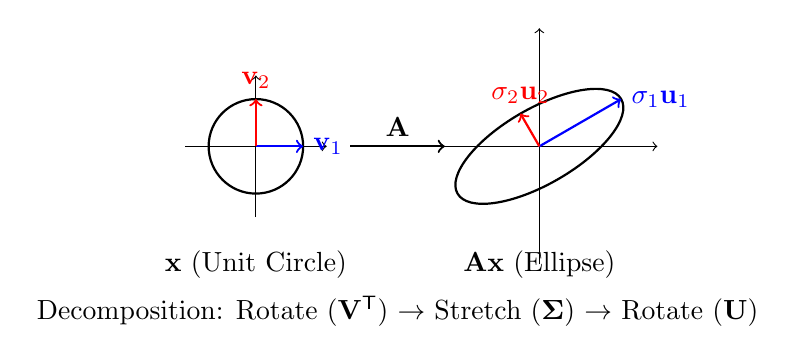
\begin{tikzpicture}[scale=0.6]
    % V^T: Rotation
    \begin{scope}[xshift=0cm]
      \draw[->] (-1.5,0) -- (1.5,0);
      \draw[->] (0,-1.5) -- (0,1.5);
      \draw[thick] (0,0) circle (1cm);
      \draw[->, blue, thick] (0,0) -- (1,0) node[right] {$\mathbf{v}_1$};
      \draw[->, red, thick] (0,0) -- (0,1) node[above] {$\mathbf{v}_2$};
      \node at (0,-2.5) {$\mathbf{x}$ (Unit Circle)};
    \end{scope}

    \draw[->, thick] (2,0) -- (4,0) node[midway, above] {$\mathbf{A}$};

    % U Sigma: Final Ellipse
    \begin{scope}[xshift=6cm]
      \draw[->] (-2.5,0) -- (2.5,0);
      \draw[->] (0,-2.5) -- (0,2.5);
      \draw[thick, rotate=30] (0,0) ellipse (2cm and 0.8cm);
      \draw[->, blue, thick, rotate=30] (0,0) -- (2,0) node[right] {$\sigma_1 \mathbf{u}_1$};
      \draw[->, red, thick, rotate=30] (0,0) -- (0,0.8) node[above] {$\sigma_2 \mathbf{u}_2$};
      \node at (0,-2.5) {$\mathbf{Ax}$ (Ellipse)};
    \end{scope}

    \node at (3,-3.5) {Decomposition: Rotate ($\mathbf{V}^{\mathsf{T}}$) $\to$ Stretch ($\mathbf{\Sigma}$) $\to$ Rotate ($\mathbf{U}$)};
  \end{tikzpicture}
\end{center}

\begin{remark}[Thin SVD]
  For computational purposes, we often use the \emph{thin} (or \emph{reduced}) SVD. If $m \geq n$ and $\operatorname{rank}(\mathbf{A}) = r$, write
  \[
    \mathbf{A} = \mathbf{U}_r \mathbf{\Sigma}_r \mathbf{V}_r^{\mathsf{T}},
  \]
  where $\mathbf{U}_r \in \mathbb{R}^{m \times r}$ contains the first $r$ columns of $\mathbf{U}$, $\mathbf{\Sigma}_r = \operatorname{diag}(\sigma_1,\dots,\sigma_r) \in \mathbb{R}^{r \times r}$, and $\mathbf{V}_r \in \mathbb{R}^{n \times r}$ contains the first $r$ columns of $\mathbf{V}$.
\end{remark}

\begin{proposition}[Connection between SVD and eigenvalues]
  Let $\mathbf{A} = \mathbf{U}\mathbf{\Sigma}\mathbf{V}^{\mathsf{T}}$ be the SVD of $\mathbf{A} \in \mathbb{R}^{m \times n}$ with singular values $\sigma_1,\dots,\sigma_r$. Then:
  \begin{enumerate}
    \item The eigenvalues of $\mathbf{A}^{\mathsf{T}}\mathbf{A}$ are $\sigma_1^2,\dots,\sigma_r^2, 0,\dots,0$, with eigenvectors given by the columns of $\mathbf{V}$.
    \item The eigenvalues of $\mathbf{A}\mathbf{A}^{\mathsf{T}}$ are $\sigma_1^2,\dots,\sigma_r^2, 0,\dots,0$, with eigenvectors given by the columns of $\mathbf{U}$.
    \item $\|\mathbf{A}\|_F^2 = \sigma_1^2 + \cdots + \sigma_r^2$.
  \end{enumerate}
\end{proposition}

\begin{proof}
  (1) From the SVD:
  \begin{align*}
    \mathbf{A}^{\mathsf{T}}\mathbf{A}
     & = (\mathbf{U}\mathbf{\Sigma}\mathbf{V}^{\mathsf{T}})^{\mathsf{T}}(\mathbf{U}\mathbf{\Sigma}\mathbf{V}^{\mathsf{T}})                   \\
     & = \mathbf{V}\mathbf{\Sigma}^{\mathsf{T}}\mathbf{U}^{\mathsf{T}}\mathbf{U}\mathbf{\Sigma}\mathbf{V}^{\mathsf{T}}                       \\
     & = \mathbf{V}\mathbf{\Sigma}^{\mathsf{T}}\mathbf{\Sigma}\mathbf{V}^{\mathsf{T}} = \mathbf{V} \mathbf{\Lambda} \mathbf{V}^{\mathsf{T}},
  \end{align*}
  where $\mathbf{\Lambda} = \mathbf{\Sigma}^{\mathsf{T}}\mathbf{\Sigma} = \operatorname{diag}(\sigma_1^2,\dots,\sigma_r^2, 0,\dots,0)$.

  (2) Similarly, $\mathbf{A}\mathbf{A}^{\mathsf{T}} = \mathbf{U}\mathbf{\Sigma}\mathbf{\Sigma}^{\mathsf{T}}\mathbf{U}^{\mathsf{T}}$ with the same eigenvalues.

  (3) By Proposition~\ref{prop:frobenius-trace}:
  \[
    \|\mathbf{A}\|_F^2 = \operatorname{tr}(\mathbf{A}^{\mathsf{T}}\mathbf{A}) = \operatorname{tr}(\mathbf{V}\mathbf{\Lambda}\mathbf{V}^{\mathsf{T}}) = \operatorname{tr}(\mathbf{\Lambda}) = \sum_{i=1}^{r} \sigma_i^2.
  \]
\end{proof}

\subsection{Applications of Singular Value Decomposition}

\subsubsection{Low-Rank Matrix Approximation (Image Compression)}
The Eckart-Young theorem states that the best rank-$k$ approximation to a matrix $\mathbf{A}$ (in the Frobenius norm sense) is given by the truncated SVD:
\[
  \mathbf{A}_k = \sum_{i=1}^{k} \sigma_i \mathbf{u}_i \mathbf{v}_i^{\mathsf{T}}.
\]
This property is fundamental to lossy data compression. Consider a grayscale image represented as a matrix $\mathbf{A} \in \mathbb{R}^{m \times n}$. By computing the SVD and storing only the first $k$ singular values and corresponding singular vectors, we can reconstruct the image with an approximation error of $\sum_{i=k+1}^{\min(m,n)} \sigma_i^2$.

For large matrices, $k \ll \min(m,n)$ is often sufficient to capture the visual structure. The storage requirement drops from $mn$ entries to $k(m+n+1)$, yielding significant compression ratios.

\subsubsection{The Moore-Penrose Pseudoinverse}
For a system of linear equations $\mathbf{A}\mathbf{x} = \mathbf{b}$, if $\mathbf{A}$ is not invertible (e.g., rectangular or singular), there is no unique solution. The \emph{pseudoinverse} $\mathbf{A}^+$ provides the "best" solution in a least-squares sense.

Using the SVD $\mathbf{A} = \mathbf{U}\mathbf{\Sigma}\mathbf{V}^{\mathsf{T}}$, the pseudoinverse is defined as:
\[
  \mathbf{A}^+ = \mathbf{V}\mathbf{\Sigma}^+\mathbf{U}^{\mathsf{T}},
\]
where $\mathbf{\Sigma}^+$ is obtained by taking the reciprocal of non-zero singular values and transposing the matrix. The solution $\mathbf{x}^* = \mathbf{A}^+\mathbf{b}$ minimizes $\|\mathbf{A}\mathbf{x} - \mathbf{b}\|_2$, and among all such minimizers, it has the smallest norm $\|\mathbf{x}\|_2$. This is widely used in solving ill-posed inverse problems in physics and engineering.

\section{Principal Component Analysis}

\subsection{The Geometric Problem}

Principal Component Analysis (PCA) solves a fundamental geometric problem: given data points in high-dimensional space, find the best low-dimensional linear subspace that approximates them.

\textbf{The problem}: Given data points $\mathbf{x}_1,\dots,\mathbf{x}_N \in \mathbb{R}^d$ (assumed centered: $\sum_{i=1}^{N}\mathbf{x}_i = \mathbf{0}$), find a $k$-dimensional linear subspace $S \subseteq \mathbb{R}^d$ that minimizes the total squared distance from all points to $S$:
\begin{equation}\label{eq:pca-geometric}
  \min_{\substack{S \subseteq \mathbb{R}^d \\ \dim(S) = k}} \sum_{i=1}^{N} \operatorname{dist}(\mathbf{x}_i, S)^2,
\end{equation}
where $\operatorname{dist}(\mathbf{x}, S) := \inf_{\mathbf{y} \in S} \|\mathbf{x} - \mathbf{y}\|_2$ is the distance from $\mathbf{x}$ to $S$.

\begin{center}
  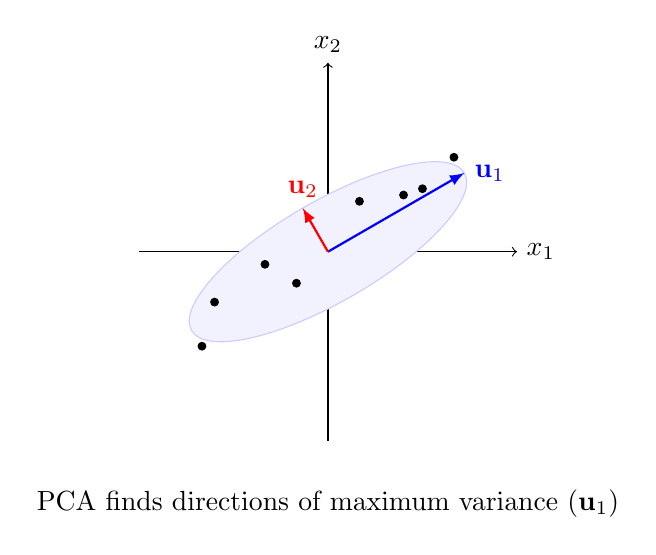
\begin{tikzpicture}[scale=0.8]
    \draw[->] (-3,0) -- (3,0) node[right] {$x_1$};
    \draw[->] (0,-3) -- (0,3) node[above] {$x_2$};

    % Ellipse of data
    \draw[rotate=30, blue!20, fill=blue!5] (0,0) ellipse (2.5 and 0.8);

    % Principal axes
    \draw[->, thick, blue, -latex, rotate=30] (0,0) -- (2.5,0) node[right] {$\mathbf{u}_1$};
    \draw[->, thick, red, -latex, rotate=30] (0,0) -- (0,0.8) node[above] {$\mathbf{u}_2$};

    % Random points (simulated)
    \foreach \x/\y in {1.5/1, 2/1.5, -1/-0.2, -2/-1.5, 0.5/0.8, -0.5/-0.5, 1.2/0.9, -1.8/-0.8} {
        \fill[black] (\x,\y) circle (2pt);
      }

    \node at (0,-4) {PCA finds directions of maximum variance ($\mathbf{u}_1$)};
  \end{tikzpicture}
\end{center}

\subsection{Parametrizing Subspaces via Orthonormal Bases}

To solve \eqref{eq:pca-geometric}, we need to parametrize $k$-dimensional subspaces. The key is to represent each subspace by an orthonormal basis.

\begin{lemma}[Orthonormal basis representation]\label{lem:subspace-parametrization}
  Let $S \subseteq \mathbb{R}^d$ be a $k$-dimensional linear subspace. Then there exists a matrix $\mathbf{W} \in \mathbb{R}^{d \times k}$ with columns $\mathbf{w}_1,\dots,\mathbf{w}_k$ such that:
  \begin{enumerate}
    \item The columns of $\mathbf{W}$ form an orthonormal basis of $S$: $\mathbf{W}^{\mathsf{T}}\mathbf{W} = \mathbf{I}_k$.
    \item $S = \operatorname{span}(\mathbf{w}_1,\dots,\mathbf{w}_k) = \{\mathbf{W}\mathbf{z} : \mathbf{z} \in \mathbb{R}^k\}$.
  \end{enumerate}
  Conversely, any $\mathbf{W} \in \mathbb{R}^{d \times k}$ with $\mathbf{W}^{\mathsf{T}}\mathbf{W} = \mathbf{I}_k$ defines a $k$-dimensional subspace $S = \operatorname{span}(\mathbf{w}_1,\dots,\mathbf{w}_k)$.
\end{lemma}

\begin{proof}
  Pick any basis of $S$ and apply Gram--Schmidt to obtain orthonormal vectors $\mathbf{w}_1,\dots,\mathbf{w}_k \in \mathbb{R}^d$.
  Let $\mathbf{W} = [\mathbf{w}_1 \mid \cdots \mid \mathbf{w}_k]$. Then $\mathbf{W}^{\mathsf{T}}\mathbf{W} = \mathbf{I}_k$ and $\operatorname{span}(\mathbf{w}_1,\dots,\mathbf{w}_k) = S$.
  Conversely, if $\mathbf{W}^{\mathsf{T}}\mathbf{W} = \mathbf{I}_k$, the columns are orthonormal, hence linearly independent, so the span has dimension $k$.
\end{proof}

Thus we can optimize over matrices $\mathbf{W} \in \mathbb{R}^{d \times k}$ with $\mathbf{W}^{\mathsf{T}}\mathbf{W} = \mathbf{I}_k$ instead of over abstract subspaces.

\subsection{Distance to a Subspace and Projection}

\begin{lemma}[Projection formula]\label{lem:projection-formula}
  Let $\mathbf{W} \in \mathbb{R}^{d \times k}$ with columns $\mathbf{w}_1,\dots,\mathbf{w}_k$ satisfying $\mathbf{W}^{\mathsf{T}}\mathbf{W} = \mathbf{I}_k$, and let $S = \operatorname{span}(\mathbf{w}_1,\dots,\mathbf{w}_k)$.
  For $\mathbf{x} \in \mathbb{R}^d$, the point in $S$ closest to $\mathbf{x}$ is
  \begin{equation}\label{eq:projection}
    \widehat{\mathbf{x}} = \mathbf{W}\mathbf{W}^{\mathsf{T}}\mathbf{x} \in \mathbb{R}^d,
  \end{equation}
  and the squared distance is
  \begin{equation}
    \operatorname{dist}(\mathbf{x}, S)^2 = \|\mathbf{x} - \mathbf{W}\mathbf{W}^{\mathsf{T}}\mathbf{x}\|^2.
  \end{equation}
\end{lemma}

\begin{proof}
  The distance to $S$ is
  \[
    \operatorname{dist}(\mathbf{x}, S) = \inf_{\mathbf{y} \in S} \|\mathbf{x} - \mathbf{y}\| = \inf_{\mathbf{z} \in \mathbb{R}^k} \|\mathbf{x} - \mathbf{W}\mathbf{z}\|,
  \]
  since every $\mathbf{y} \in S$ can be written as $\mathbf{W}\mathbf{z}$ for some $\mathbf{z} \in \mathbb{R}^k$.

  Define $f(\mathbf{z}) = \|\mathbf{x} - \mathbf{W}\mathbf{z}\|^2 = (\mathbf{x} - \mathbf{W}\mathbf{z})^{\mathsf{T}}(\mathbf{x} - \mathbf{W}\mathbf{z})$. Expanding:
  \[
    f(\mathbf{z}) = \mathbf{x}^{\mathsf{T}}\mathbf{x} - 2\mathbf{x}^{\mathsf{T}}\mathbf{W}\mathbf{z} + \mathbf{z}^{\mathsf{T}}\mathbf{W}^{\mathsf{T}}\mathbf{W}\mathbf{z}.
  \]
  Using $\mathbf{W}^{\mathsf{T}}\mathbf{W} = \mathbf{I}_k$:
  \[
    f(\mathbf{z}) = \mathbf{x}^{\mathsf{T}}\mathbf{x} - 2\mathbf{x}^{\mathsf{T}}\mathbf{W}\mathbf{z} + \mathbf{z}^{\mathsf{T}}\mathbf{z}.
  \]
  Taking the gradient: $\nabla_{\mathbf{z}} f = -2\mathbf{W}^{\mathsf{T}}\mathbf{x} + 2\mathbf{z}$. Setting to zero gives $\mathbf{z}^* = \mathbf{W}^{\mathsf{T}}\mathbf{x}$.
  The Hessian is $2\mathbf{I}_k$, which is positive definite, so this is the unique global minimizer.

  Thus $\widehat{\mathbf{x}} = \mathbf{W}\mathbf{z}^* = \mathbf{W}\mathbf{W}^{\mathsf{T}}\mathbf{x}$, and
  \[
    \operatorname{dist}(\mathbf{x}, S)^2 = \|\mathbf{x} - \mathbf{W}\mathbf{W}^{\mathsf{T}}\mathbf{x}\|^2.
  \]
\end{proof}

\begin{remark}
  The matrix $\mathbf{P} = \mathbf{W}\mathbf{W}^{\mathsf{T}} \in \mathbb{R}^{d \times d}$ is the orthogonal projection onto $S$. It is symmetric, idempotent ($\mathbf{P}^2 = \mathbf{P}$), and has rank $k$.
  The coordinate vector of $\widehat{\mathbf{x}}$ in the basis given by columns of $\mathbf{W}$ is $\mathbf{z}^* = \mathbf{W}^{\mathsf{T}}\mathbf{x} \in \mathbb{R}^k$.

  \begin{center}
    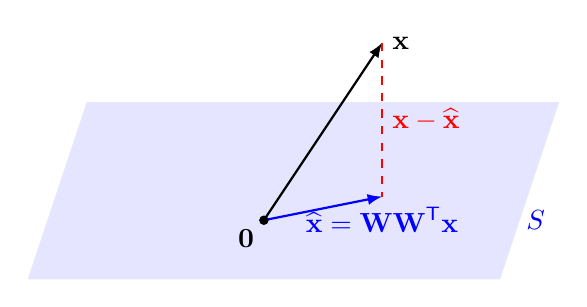
\begin{tikzpicture}[scale=1.5]
      % Plane
      \fill[blue!10] (-2,-0.5) -- (2,-0.5) -- (2.5,1) -- (-1.5,1) -- cycle;
      \node[blue] at (2.3,0) {$S$};

      % Vectors
      \coordinate (O) at (0,0);
      \coordinate (X) at (1,1.5);
      \coordinate (P) at (1,0.2);

      \draw[->, thick, -latex] (O) -- (X) node[right] {$\mathbf{x}$};
      \draw[->, thick, -latex, blue] (O) -- (P) node[below] {$\widehat{\mathbf{x}} = \mathbf{WW}^{\mathsf{T}}\mathbf{x}$};
      \draw[dashed, red, thick] (X) -- (P) node[midway, right] {$\mathbf{x} - \widehat{\mathbf{x}}$};

      % Origin
      \filldraw (O) circle (1pt) node[below left] {$\mathbf{0}$};
    \end{tikzpicture}
  \end{center}
\end{remark}
\subsection{The Matrix Optimization Problem}

\begin{definition}[Sample covariance matrix]
  Given centered data $\mathbf{x}_1,\dots,\mathbf{x}_N \in \mathbb{R}^d$, the \emph{sample covariance matrix} is
  \begin{equation}
    \mathbf{C} = \frac{1}{N} \sum_{i=1}^{N} \mathbf{x}_i \mathbf{x}_i^{\mathsf{T}} \in \mathbb{R}^{d \times d}.
  \end{equation}
  It is symmetric and positive semidefinite.
\end{definition}

\begin{theorem}[PCA solution]\label{thm:pca}
  Let $\mathbf{x}_1,\dots,\mathbf{x}_N \in \mathbb{R}^d$ be centered data with covariance matrix $\mathbf{C}$.
  Let $\mathbf{C} = \mathbf{U}\mathbf{\Lambda}\mathbf{U}^{\mathsf{T}}$ be the spectral decomposition with eigenvalues $\lambda_1 \geq \lambda_2 \geq \cdots \geq \lambda_d \geq 0$ and corresponding eigenvectors $\mathbf{u}_1,\dots,\mathbf{u}_d$.

  The geometric optimization problem \eqref{eq:pca-geometric} is equivalent to:
  \begin{equation}\label{eq:pca-trace}
    \min_{\substack{\mathbf{W} \in \mathbb{R}^{d \times k} \\ \mathbf{W}^{\mathsf{T}}\mathbf{W} = \mathbf{I}_k}} \sum_{i=1}^{N} \|\mathbf{x}_i - \mathbf{W}\mathbf{W}^{\mathsf{T}}\mathbf{x}_i\|^2 \quad \Leftrightarrow \quad \max_{\substack{\mathbf{W} \in \mathbb{R}^{d \times k} \\ \mathbf{W}^{\mathsf{T}}\mathbf{W} = \mathbf{I}_k}} \operatorname{tr}(\mathbf{W}^{\mathsf{T}}\mathbf{C}\mathbf{W}).
  \end{equation}

  \textbf{Solution}: The optimal subspace is $S^* = \operatorname{span}(\mathbf{u}_1,\dots,\mathbf{u}_k)$, spanned by the top $k$ eigenvectors of $\mathbf{C}$.
  Any optimal $\mathbf{W}^*$ has the form
  \begin{equation}
    \mathbf{W}^* = [\mathbf{u}_1 \mid \cdots \mid \mathbf{u}_k] \mathbf{R},
  \end{equation}
  where $\mathbf{R} \in \mathbb{R}^{k \times k}$ is any orthogonal matrix. The minimum reconstruction error is
  \begin{equation}
    \sum_{i=1}^{N} \operatorname{dist}(\mathbf{x}_i, S^*)^2 = N \sum_{j=k+1}^{d} \lambda_j.
  \end{equation}
\end{theorem}

\begin{proof}
  \textbf{Step 1: From geometric problem to Frobenius norm.}

  By Lemma~\ref{lem:projection-formula}, for $S = \operatorname{span}(\mathbf{w}_1,\dots,\mathbf{w}_k)$ where $\mathbf{W} = [\mathbf{w}_1 \mid \cdots \mid \mathbf{w}_k]$ we have
  \[
    \sum_{i=1}^{N} \operatorname{dist}(\mathbf{x}_i, S)^2 = \sum_{i=1}^{N} \|\mathbf{x}_i - \mathbf{W}\mathbf{W}^{\mathsf{T}}\mathbf{x}_i\|^2.
  \]

  Let $\mathbf{X} \in \mathbb{R}^{N \times d}$ be the data matrix with rows $\mathbf{x}_i^{\mathsf{T}}$. Then
  \[
    \sum_{i=1}^{N} \|\mathbf{x}_i - \mathbf{W}\mathbf{W}^{\mathsf{T}}\mathbf{x}_i\|^2 = \|\mathbf{X} - \mathbf{X}\mathbf{W}\mathbf{W}^{\mathsf{T}}\|_F^2,
  \]
  where $\|\cdot\|_F$ is the Frobenius norm.

  \textbf{Step 2: Converting to trace maximization.}

  Expand the Frobenius norm using $\|\mathbf{A}\|_F^2 = \operatorname{tr}(\mathbf{A}^{\mathsf{T}}\mathbf{A})$:
  \begin{align*}
    \|\mathbf{X} - \mathbf{X}\mathbf{W}\mathbf{W}^{\mathsf{T}}\|_F^2
     & = \operatorname{tr}\left((\mathbf{X} - \mathbf{X}\mathbf{W}\mathbf{W}^{\mathsf{T}})^{\mathsf{T}}(\mathbf{X} - \mathbf{X}\mathbf{W}\mathbf{W}^{\mathsf{T}})\right)                                                                                                                                                                                                \\
     & = \operatorname{tr}(\mathbf{X}^{\mathsf{T}}\mathbf{X}) - \operatorname{tr}(\mathbf{X}^{\mathsf{T}}\mathbf{X}\mathbf{W}\mathbf{W}^{\mathsf{T}}) - \operatorname{tr}(\mathbf{W}\mathbf{W}^{\mathsf{T}}\mathbf{X}^{\mathsf{T}}\mathbf{X}) + \operatorname{tr}(\mathbf{W}\mathbf{W}^{\mathsf{T}}\mathbf{X}^{\mathsf{T}}\mathbf{X}\mathbf{W}\mathbf{W}^{\mathsf{T}}).
  \end{align*}

  Using the cyclic property of trace, $\operatorname{tr}(\mathbf{A}\mathbf{B}\mathbf{C}) = \operatorname{tr}(\mathbf{C}\mathbf{A}\mathbf{B})$:
  \begin{align*}
    \operatorname{tr}(\mathbf{X}^{\mathsf{T}}\mathbf{X}\mathbf{W}\mathbf{W}^{\mathsf{T}})                                  & = \operatorname{tr}(\mathbf{W}^{\mathsf{T}}\mathbf{X}^{\mathsf{T}}\mathbf{X}\mathbf{W}),                                                                                                                                 \\
    \operatorname{tr}(\mathbf{W}\mathbf{W}^{\mathsf{T}}\mathbf{X}^{\mathsf{T}}\mathbf{X})                                  & = \operatorname{tr}(\mathbf{W}^{\mathsf{T}}\mathbf{X}^{\mathsf{T}}\mathbf{X}\mathbf{W}),                                                                                                                                 \\
    \operatorname{tr}(\mathbf{W}\mathbf{W}^{\mathsf{T}}\mathbf{X}^{\mathsf{T}}\mathbf{X}\mathbf{W}\mathbf{W}^{\mathsf{T}}) & = \operatorname{tr}(\mathbf{W}^{\mathsf{T}}\mathbf{X}^{\mathsf{T}}\mathbf{X}\mathbf{W} \cdot \mathbf{W}^{\mathsf{T}}\mathbf{W}) = \operatorname{tr}(\mathbf{W}^{\mathsf{T}}\mathbf{X}^{\mathsf{T}}\mathbf{X}\mathbf{W}),
  \end{align*}
  where the last equality uses $\mathbf{W}^{\mathsf{T}}\mathbf{W} = \mathbf{I}_k$. Thus:
  \[
    \|\mathbf{X} - \mathbf{X}\mathbf{W}\mathbf{W}^{\mathsf{T}}\|_F^2 = \operatorname{tr}(\mathbf{X}^{\mathsf{T}}\mathbf{X}) - \operatorname{tr}(\mathbf{W}^{\mathsf{T}}\mathbf{X}^{\mathsf{T}}\mathbf{X}\mathbf{W}).
  \]

  Since $\operatorname{tr}(\mathbf{X}^{\mathsf{T}}\mathbf{X})$ is constant, minimizing reconstruction error is equivalent to maximizing $\operatorname{tr}(\mathbf{W}^{\mathsf{T}}\mathbf{X}^{\mathsf{T}}\mathbf{X}\mathbf{W})$.
  Define $\mathbf{C} = \frac{1}{N}\mathbf{X}^{\mathsf{T}}\mathbf{X}$. Then \eqref{eq:pca-geometric} becomes:
  \[
    \max_{\substack{\mathbf{W} \in \mathbb{R}^{d \times k} \\ \mathbf{W}^{\mathsf{T}}\mathbf{W} = \mathbf{I}_k}} \operatorname{tr}(\mathbf{W}^{\mathsf{T}}\mathbf{C}\mathbf{W}).
  \]

  \textbf{Step 3: Change of variables to eigenvector basis.}

  By the spectral theorem, $\mathbf{C} = \mathbf{U}\mathbf{\Lambda}\mathbf{U}^{\mathsf{T}}$ with $\mathbf{U}^{\mathsf{T}}\mathbf{U} = \mathbf{I}_d$ and $\mathbf{\Lambda} = \operatorname{diag}(\lambda_1,\dots,\lambda_d)$, $\lambda_1 \geq \cdots \geq \lambda_d \geq 0$.

  Define $\mathbf{S} := \mathbf{U}^{\mathsf{T}}\mathbf{W} \in \mathbb{R}^{d \times k}$. Since $\mathbf{U}$ is orthogonal, $\mathbf{S}^{\mathsf{T}}\mathbf{S} = \mathbf{W}^{\mathsf{T}}\mathbf{U}\mathbf{U}^{\mathsf{T}}\mathbf{W} = \mathbf{I}_k$.
  Moreover,
  \[
    \operatorname{tr}(\mathbf{W}^{\mathsf{T}}\mathbf{C}\mathbf{W}) = \operatorname{tr}(\mathbf{W}^{\mathsf{T}}\mathbf{U}\mathbf{\Lambda}\mathbf{U}^{\mathsf{T}}\mathbf{W}) = \operatorname{tr}(\mathbf{S}^{\mathsf{T}}\mathbf{\Lambda}\mathbf{S}) = \sum_{i=1}^{d} \lambda_i \sum_{j=1}^{k} s_{ij}^2.
  \]

  \textbf{Step 4: Optimization over $\mathbf{S}$.}

  The constraint $\mathbf{S}^{\mathsf{T}}\mathbf{S} = \mathbf{I}_k$ implies $\sum_{i=1}^{d} s_{ij}^2 = 1$ for each column $j$, hence $\sum_{i=1}^{d} \sum_{j=1}^{k} s_{ij}^2 = k$.

  Define $\alpha_i := \sum_{j=1}^{k} s_{ij}^2 \in [0, k]$, the total squared mass in row $i$. Then $\sum_{i=1}^{d} \alpha_i = k$ and
  \[
    \operatorname{tr}(\mathbf{S}^{\mathsf{T}}\mathbf{\Lambda}\mathbf{S}) = \sum_{i=1}^{d} \lambda_i \alpha_i.
  \]

  \textbf{Claim}: Under $\lambda_1 \geq \cdots \geq \lambda_d$ and $\alpha_i \geq 0$, $\sum \alpha_i = k$, we have $\sum_{i=1}^{d} \lambda_i \alpha_i \leq \sum_{i=1}^{k} \lambda_i$, with equality if and only if $\alpha_i = 1$ for $i \leq k$ and $\alpha_i = 0$ for $i > k$.

  \textit{Proof of claim}: If there exist $i \leq k < j$ with $\alpha_i < 1$ and $\alpha_j > 0$, define $\widetilde{\alpha}_i = \alpha_i + \epsilon$, $\widetilde{\alpha}_j = \alpha_j - \epsilon$ for small $\epsilon > 0$. Then
  \[
    \sum_{\ell} \lambda_{\ell} \widetilde{\alpha}_{\ell} = \sum_{\ell} \lambda_{\ell} \alpha_{\ell} + \epsilon(\lambda_i - \lambda_j) \geq \sum_{\ell} \lambda_{\ell} \alpha_{\ell},
  \]
  with strict inequality if $\lambda_i > \lambda_j$. Repeating this argument shows the maximum is $\sum_{i=1}^{k} \lambda_i$. \qed

  One feasible $\mathbf{S}$ achieving this is $\mathbf{S} = \begin{pmatrix} \mathbf{I}_k \\ \mathbf{0} \end{pmatrix}$, which gives $\mathbf{W} = \mathbf{U}\mathbf{S} = [\mathbf{u}_1 \mid \cdots \mid \mathbf{u}_k]$.

  Any other optimal $\mathbf{W}^*$ satisfies $\mathbf{U}^{\mathsf{T}}\mathbf{W}^* = \mathbf{S}'$ with the same structure, i.e., $\mathbf{S}' = \begin{pmatrix} \mathbf{R} \\ \mathbf{0} \end{pmatrix}$ for some orthogonal $\mathbf{R} \in \mathbb{R}^{k \times k}$, giving $\mathbf{W}^* = [\mathbf{u}_1 \mid \cdots \mid \mathbf{u}_k]\mathbf{R}$.

  The minimum reconstruction error is $\operatorname{tr}(\mathbf{X}^{\mathsf{T}}\mathbf{X}) - N \sum_{j=1}^{k}\lambda_j = N \sum_{j=k+1}^{d} \lambda_j$.
\end{proof}

\begin{remark}[Alternative proof via Lagrange multipliers]
  We can also solve the $k=1$ case (finding the first principal component) using Lagrange multipliers, then extend to general $k$ by deflation.

  \textbf{Finding the first principal component ($k=1$).}

  Maximize $f(\mathbf{w}) = \mathbf{w}^{\mathsf{T}}\mathbf{C}\mathbf{w}$ subject to $g(\mathbf{w}) = \mathbf{w}^{\mathsf{T}}\mathbf{w} - 1 = 0$, where $\mathbf{w} \in \mathbb{R}^d$.

  Form the Lagrangian:
  \[
    \mathcal{L}(\mathbf{w}, \lambda) = \mathbf{w}^{\mathsf{T}}\mathbf{C}\mathbf{w} - \lambda(\mathbf{w}^{\mathsf{T}}\mathbf{w} - 1).
  \]

  Take the gradient with respect to $\mathbf{w}$ and set to zero:
  \[
    \nabla_{\mathbf{w}} \mathcal{L} = 2\mathbf{C}\mathbf{w} - 2\lambda\mathbf{w} = \mathbf{0} \quad \Rightarrow \quad \mathbf{C}\mathbf{w} = \lambda\mathbf{w}.
  \]

  So $\mathbf{w}$ must be an eigenvector of $\mathbf{C}$ with eigenvalue $\lambda$. The objective value at this critical point is:
  \[
    f(\mathbf{w}) = \mathbf{w}^{\mathsf{T}}\mathbf{C}\mathbf{w} = \mathbf{w}^{\mathsf{T}}(\lambda\mathbf{w}) = \lambda \mathbf{w}^{\mathsf{T}}\mathbf{w} = \lambda.
  \]

  To maximize variance, choose $\mathbf{w} = \mathbf{u}_1$, the eigenvector corresponding to the largest eigenvalue $\lambda_1$.

  \textbf{Finding subsequent components ($k \geq 2$).}

  For the $j$-th principal component with $j > 1$, maximize $\mathbf{w}^{\mathsf{T}}\mathbf{C}\mathbf{w}$ subject to:
  \begin{itemize}
    \item $\mathbf{w}^{\mathsf{T}}\mathbf{w} = 1$ (unit norm),
    \item $\mathbf{w}^{\mathsf{T}}\mathbf{u}_i = 0$ for all $i < j$ (orthogonal to previous components).
  \end{itemize}

  Form the Lagrangian with multiple constraints:
  \[
    \mathcal{L}(\mathbf{w}, \lambda, \mu_1,\dots,\mu_{j-1}) = \mathbf{w}^{\mathsf{T}}\mathbf{C}\mathbf{w} - \lambda(\mathbf{w}^{\mathsf{T}}\mathbf{w} - 1) - \sum_{i=1}^{j-1} \mu_i \mathbf{w}^{\mathsf{T}}\mathbf{u}_i.
  \]

  Taking the gradient:
  \[
    \nabla_{\mathbf{w}} \mathcal{L} = 2\mathbf{C}\mathbf{w} - 2\lambda\mathbf{w} - \sum_{i=1}^{j-1} \mu_i \mathbf{u}_i = \mathbf{0}.
  \]

  Multiply on the left by $\mathbf{u}_i^{\mathsf{T}}$ for any $i < j$:
  \[
    2\mathbf{u}_i^{\mathsf{T}}\mathbf{C}\mathbf{w} - 2\lambda \mathbf{u}_i^{\mathsf{T}}\mathbf{w} - \mu_i = 0.
  \]
  Using $\mathbf{u}_i^{\mathsf{T}}\mathbf{w} = 0$ (orthogonality constraint) and $\mathbf{C}\mathbf{u}_i = \lambda_i \mathbf{u}_i$ (since $\mathbf{u}_i$ is an eigenvector):
  \[
    2(\mathbf{C}\mathbf{u}_i)^{\mathsf{T}}\mathbf{w} - \mu_i = 2\lambda_i \mathbf{u}_i^{\mathsf{T}}\mathbf{w} - \mu_i = -\mu_i = 0.
  \]
  So $\mu_i = 0$ for all $i < j$. This reduces the stationarity condition to:
  \[
    \mathbf{C}\mathbf{w} = \lambda\mathbf{w}.
  \]

  Again, $\mathbf{w}$ must be an eigenvector. Combined with the orthogonality constraints $\mathbf{w}^{\mathsf{T}}\mathbf{u}_i = 0$ for $i < j$, we have $\mathbf{w} \in \operatorname{span}(\mathbf{u}_j,\mathbf{u}_{j+1},\dots,\mathbf{u}_d)$. To maximize the objective $\lambda$, choose $\mathbf{w} = \mathbf{u}_j$ with eigenvalue $\lambda_j$.

  By induction, the first $k$ principal components are $\mathbf{u}_1,\dots,\mathbf{u}_k$.
\end{remark}

\begin{remark}[Connection between PCA and SVD]\label{rem:pca-svd}
  PCA can be computed directly using SVD without forming the covariance matrix.

  Let $\mathbf{X} \in \mathbb{R}^{N \times d}$ be the centered data matrix with rows $\mathbf{x}_i^{\mathsf{T}}$. Compute the thin SVD:
  \[
    \mathbf{X} = \mathbf{U}_X \mathbf{\Sigma} \mathbf{V}^{\mathsf{T}},
  \]
  where $\mathbf{U}_X \in \mathbb{R}^{N \times r}$, $\mathbf{\Sigma} = \operatorname{diag}(\sigma_1,\dots,\sigma_r) \in \mathbb{R}^{r \times r}$, and $\mathbf{V} \in \mathbb{R}^{d \times r}$ with $r = \operatorname{rank}(\mathbf{X})$.

  The covariance matrix is:
  \[
    \mathbf{C} = \frac{1}{N}\mathbf{X}^{\mathsf{T}}\mathbf{X} = \frac{1}{N}\mathbf{V}\mathbf{\Sigma}^{\mathsf{T}}\mathbf{U}_X^{\mathsf{T}}\mathbf{U}_X\mathbf{\Sigma}\mathbf{V}^{\mathsf{T}} = \frac{1}{N}\mathbf{V}\mathbf{\Sigma}^2\mathbf{V}^{\mathsf{T}}.
  \]

  Comparing with the spectral decomposition $\mathbf{C} = \mathbf{U}\mathbf{\Lambda}\mathbf{U}^{\mathsf{T}}$, we see:
  \begin{itemize}
    \item \textbf{Principal components}: The columns of $\mathbf{V}$ are the principal components (eigenvectors of $\mathbf{C}$).
    \item \textbf{Eigenvalues}: $\lambda_i = \frac{\sigma_i^2}{N}$ for $i = 1,\dots,r$.
    \item \textbf{Variance explained}: The variance captured by the $i$-th principal component is $\frac{\sigma_i^2}{N}$.
  \end{itemize}

  \textbf{Computational advantage}: Computing SVD of $\mathbf{X} \in \mathbb{R}^{N \times d}$ is often faster and more numerically stable than forming $\mathbf{C} = \mathbf{X}^{\mathsf{T}}\mathbf{X} \in \mathbb{R}^{d \times d}$ and computing its eigendecomposition, especially when $N \gg d$ or $d \gg N$.
\end{remark}

\begin{corollary}[PCA algorithm]
  To perform PCA on centered data $\mathbf{x}_1,\dots,\mathbf{x}_N \in \mathbb{R}^d$:
  \begin{enumerate}
    \item Compute the covariance matrix $\mathbf{\Sigma} = \frac{1}{N}\sum_{i=1}^{N} \mathbf{x}_i\mathbf{x}_i^{\mathsf{T}}$.
    \item Find the eigenvalue decomposition $\mathbf{\Sigma} = \mathbf{U}\mathbf{\Lambda}\mathbf{U}^{\mathsf{T}}$.
    \item The principal components are the columns of $\mathbf{U}$, ordered by decreasing eigenvalue.
    \item To project onto $k$ dimensions, use $\mathbf{W} = [\mathbf{u}_1 \mid \cdots \mid \mathbf{u}_k]$ and compute $\mathbf{z}_i = \mathbf{W}^{\mathsf{T}}\mathbf{x}_i$.
  \end{enumerate}
  The variance explained by the first $k$ components is $\frac{\sum_{i=1}^{k}\lambda_i}{\sum_{i=1}^{d}\lambda_i}$.
\end{corollary}

\subsection{Applications of Principal Component Analysis}

\subsubsection{Dimensionality Reduction in Images (Eigenfaces)}
Natural images, such as faces, are high-dimensional data points. A $256 \times 256$ grayscale image corresponds to a vector $\mathbf{x} \in \mathbb{R}^{65536}$. However, the space of "valid" face images is a much lower-dimensional manifold within this huge space.

PCA identifies the principal directions of variation in the dataset of face images. The eigenvectors $\mathbf{u}_1, \dots, \mathbf{u}_k$ of the covariance matrix are called \emph{eigenfaces}. They represent the fundamental "ghost-like" features (such as lighting direction, face shape, or pose) from which any specific face can be constructed.

By keeping only the top $k \approx 100$ eigenfaces, we can compress the image $\mathbf{x}$ into a coefficient vector $\mathbf{z} \in \mathbb{R}^{100}$:
\[
  \mathbf{z} = \mathbf{W}^{\mathsf{T}}(\mathbf{x} - \boldsymbol{\mu}),
\]
where $\boldsymbol{\mu}$ is the mean face and $\mathbf{W} = [\mathbf{u}_1 \mid \dots \mid \mathbf{u}_k]$. The reconstruction $\widehat{\mathbf{x}} = \boldsymbol{\mu} + \mathbf{W}\mathbf{z}$ preserves the essential facial features while discarding noise and minor variations, achieving a compression ratio of over 600:1.

\subsubsection{Feature Engineering in Recommender Systems}
In a recommender system, we have a sparse user-item interaction matrix $\mathbf{R} \in \mathbb{R}^{N \times M}$, where $R_{ij}$ represents the rating user $i$ gives to item $j$. The goal is to predict missing ratings.

PCA (or more precisely, SVD-based matrix factorization) transforms this sparse matrix into dense low-dimensional embeddings. We assume that user preferences depend on a small number of latent factors (e.g., for movies: "action vs. drama", "serious vs. comedy").

By approximating the matrix $\mathbf{R}$ with a rank-$k$ matrix, we map each user $i$ to a vector $\mathbf{p}_i \in \mathbb{R}^k$ and each item $j$ to a vector $\mathbf{q}_j \in \mathbb{R}^k$ such that
\[
  R_{ij} \approx \mathbf{p}_i^{\mathsf{T}}\mathbf{q}_j.
\]
These latent vectors capture semantic similarities: users with similar $\mathbf{p}$ vectors share tastes, and items with similar $\mathbf{q}$ vectors are semantically related, enabling the system to recommend items that align with the user's latent preferences.

\subsubsection{Genomics and Population Genetics}
In genomics, the data matrix $\mathbf{X}$ consists of Single Nucleotide Polymorphisms (SNPs) for $N$ individuals across $d$ genetic markers (often $d \gg N$).

PCA is applied to this matrix to visualize population structure. The first two principal components often reveal geographic ancestry. For example, when applied to European populations, the projection of individuals onto the plane spanned by the first two principal components remarkably reconstructs the map of Europe, with individuals clustering by their country of origin. This indicates that geography is the dominant factor explaining genetic variation.


\section{UMAP: Nonlinear Dimensionality Reduction}

\subsection{Limitations of Linear Methods}

PCA is a powerful technique, but it has a fundamental limitation: it can only discover \emph{linear} structure in data. When data lies on or near a nonlinear manifold embedded in high-dimensional space, linear projections may fail to capture the intrinsic geometry.

\begin{example}[Swiss roll]
  Consider the ``Swiss roll'' dataset: points sampled from a 2D rectangular sheet that has been rolled up into a spiral in $\mathbb{R}^3$. The intrinsic dimensionality is 2 (points can be parameterized by their position on the original sheet), but PCA projecting to 2D will ``crush'' the roll, mixing together points that are far apart along the manifold.
\end{example}

\begin{figure}[h]
\centering
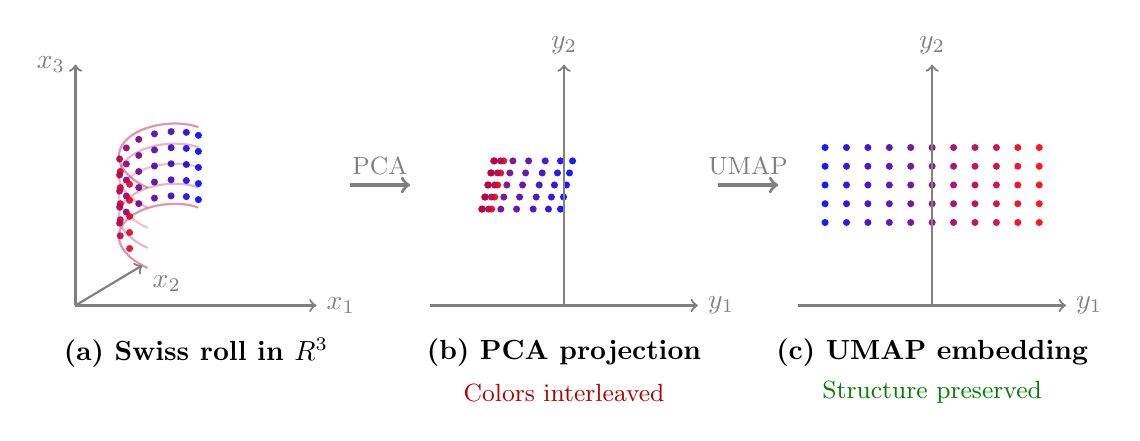
\begin{tikzpicture}[scale=0.85]
  % === LEFT: Swiss roll in 3D ===
  \begin{scope}[shift={(-5.5,0)}]
    % Draw spiral curves at different heights to show 3D structure
    \draw[thick, purple!70, opacity=0.6]
      plot[domain=1.5:4.2, samples=40, smooth]
      ({0.35*\x*cos(\x r)}, {-0.6 + 0.35*\x*sin(\x r)*0.5});
    \draw[thick, purple!50, opacity=0.6]
      plot[domain=1.5:4.2, samples=40, smooth]
      ({0.35*\x*cos(\x r)}, {-0.3 + 0.35*\x*sin(\x r)*0.5});
    \draw[thick, purple!40, opacity=0.6]
      plot[domain=1.5:4.2, samples=40, smooth]
      ({0.35*\x*cos(\x r)}, {0 + 0.35*\x*sin(\x r)*0.5});
    \draw[thick, purple!50, opacity=0.6]
      plot[domain=1.5:4.2, samples=40, smooth]
      ({0.35*\x*cos(\x r)}, {0.3 + 0.35*\x*sin(\x r)*0.5});
    \draw[thick, purple!70, opacity=0.6]
      plot[domain=1.5:4.2, samples=40, smooth]
      ({0.35*\x*cos(\x r)}, {0.6 + 0.35*\x*sin(\x r)*0.5});
    % Add points on the manifold with color gradient along the spiral
    \foreach \t in {1.5,1.8,...,4.2} {
      \foreach \h in {-0.8,-0.4,0,0.4,0.8} {
        \pgfmathsetmacro{\col}{(\t-1.5)/(4.2-1.5)*100}
        \fill[red!\col!blue, opacity=0.9]
          ({0.35*\t*cos(\t r)}, {\h*0.6 + 0.35*\t*sin(\t r)*0.5}) circle (1.5pt);
      }
    }
    % Axes
    \draw[->, thick, gray] (-1.8,-1.8) -- (1.8,-1.8) node[right] {$x_1$};
    \draw[->, thick, gray] (-1.8,-1.8) -- (-1.8,1.8) node[left] {$x_3$};
    \draw[->, thick, gray] (-1.8,-1.8) -- (-0.8,-1.2) node[below right] {$x_2$};
    % Title
    \node[font=\bfseries] at (0,-2.5) {(a) Swiss roll in $\mathbb{R}^3$};
  \end{scope}

  % === MIDDLE: PCA projection ===
  \begin{scope}[shift={(0,0)}]
    % PCA crushes the spiral - colors get mixed
    \foreach \t in {1.5,1.8,...,4.2} {
      \pgfmathsetmacro{\col}{(\t-1.5)/(4.2-1.5)*100}
      \pgfmathsetmacro{\px}{0.35*\t*cos(\t r)}
      % Points collapse vertically, spread horizontally
      \foreach \jitter in {-0.3,-0.15,0,0.15,0.3} {
        \fill[red!\col!blue, opacity=0.9]
          ({\px + \jitter*0.3}, {\jitter*1.2}) circle (1.5pt);
      }
    }
    % Axes
    \draw[->, thick, gray] (-2,-1.8) -- (2,-1.8) node[right] {$y_1$};
    \draw[->, thick, gray] (0,-1.8) -- (0,1.8) node[above] {$y_2$};
    % Title
    \node[font=\bfseries] at (0,-2.5) {(b) PCA projection};
    \node[font=\small, red!70!black] at (0,-3.1) {Colors interleaved};
  \end{scope}

  % === RIGHT: UMAP embedding ===
  \begin{scope}[shift={(5.5,0)}]
    % UMAP unrolls the manifold - color gradient preserved
    \foreach \i in {0,1,...,10} {
      \pgfmathsetmacro{\col}{\i/10*100}
      \foreach \j in {-2,-1,0,1,2} {
        \fill[red!\col!blue, opacity=0.9]
          ({-1.6 + \i*0.32}, {\j*0.28}) circle (1.5pt);
      }
    }
    % Axes
    \draw[->, thick, gray] (-2,-1.8) -- (2,-1.8) node[right] {$y_1$};
    \draw[->, thick, gray] (0,-1.8) -- (0,1.8) node[above] {$y_2$};
    % Title
    \node[font=\bfseries] at (0,-2.5) {(c) UMAP embedding};
    \node[font=\small, green!50!black] at (0,-3.1) {Structure preserved};
  \end{scope}

  % Arrows between panels
  \draw[->, very thick, gray] (-3.2,0) -- (-2.3,0) node[midway, above] {\small PCA};
  \draw[->, very thick, gray] (2.3,0) -- (3.2,0) node[midway, above] {\small UMAP};
\end{tikzpicture}
\caption{The Swiss roll problem illustrates the limitation of linear dimensionality reduction. (a) Data lies on a 2D manifold rolled into 3D; color encodes position along the manifold (blue $\to$ red). (b) PCA projects onto the plane of maximum variance, mixing together points that are far apart on the manifold (note interleaved colors). (c) UMAP recovers the intrinsic 2D structure by preserving local neighborhoods, unrolling the manifold so that color varies smoothly from left to right.}
\label{fig:swiss-roll}
\end{figure}

This motivates \emph{manifold learning} methods that can recover nonlinear structure. \textbf{UMAP} (Uniform Manifold Approximation and Projection) is a state-of-the-art technique grounded in Riemannian geometry and algebraic topology.

\subsection{Mathematical Foundations}

UMAP is built on the assumption that the data is uniformly distributed on a Riemannian manifold. The key insight is that we can infer the local metric structure from the data itself.

\subsubsection{Local Distance and the Riemannian Assumption}

Suppose data points $\mathbf{x}_1, \dots, \mathbf{x}_N$ lie on or near an unknown Riemannian manifold $\mathcal{M}$ embedded in $\mathbb{R}^d$. If the data is uniformly distributed on $\mathcal{M}$, then locally around each point $\mathbf{x}_i$, the density of nearby points reveals information about the local geometry.

For each point $\mathbf{x}_i$, UMAP constructs a \emph{local metric} by finding its $k$ nearest neighbors and defining a distance scale $\sigma_i > 0$ such that:
\begin{equation}\label{eq:umap-sigma}
  \sum_{j=1}^{k} \exp\left(-\frac{d(\mathbf{x}_i, \mathbf{x}_{i_j}) - \rho_i}{\sigma_i}\right) = \log_2(k),
\end{equation}
where $\mathbf{x}_{i_1}, \dots, \mathbf{x}_{i_k}$ are the $k$ nearest neighbors of $\mathbf{x}_i$, and $\rho_i = \min_j d(\mathbf{x}_i, \mathbf{x}_{i_j})$ is the distance to the nearest neighbor. This normalization ensures each point ``sees'' a comparable local neighborhood regardless of the local density.

\begin{remark}[On the uniformity assumption]\label{rem:umap-uniformity}
  The assumption that data is \emph{uniformly} distributed on $\mathcal{M}$ is crucial for interpreting local density as geometric information. When data is non-uniform:
  \begin{itemize}
    \item \textbf{Dense regions} will have small $\sigma_i$ values, making the algorithm treat nearby points as ``close'' on the manifold.
    \item \textbf{Sparse regions} will have large $\sigma_i$ values, stretching distances to maintain connectivity.
  \end{itemize}
  This adaptive scaling means UMAP \emph{implicitly assumes} non-uniform sampling reflects the underlying geometry (e.g., higher curvature regions sampled more densely). If the non-uniformity is purely a sampling artifact unrelated to geometry, UMAP may distort the true manifold structure. In practice, this is often acceptable because:
  \begin{enumerate}
    \item The local normalization via $\sigma_i$ partially compensates for density variations.
    \item For visualization, preserving \emph{relative} neighborhood structure matters more than exact distances.
  \end{enumerate}
\end{remark}

\begin{remark}[Embeddings on the sphere and fundamental non-uniformity]\label{rem:umap-sphere}
  A common application of UMAP is visualizing \emph{embedding vectors} from neural networks (word embeddings, sentence embeddings, image features). These are often $L^2$-normalized to lie on the unit sphere $S^{d-1} \subset \mathbb{R}^d$. Here the non-uniformity is typically \textbf{fundamental}, not a sampling artifact:
  \begin{itemize}
    \item Some semantic regions (e.g., common words, frequent image classes) are inherently more populated.
    \item The embedding space may have ``semantic voids''---regions with no meaningful concepts.
    \item Cluster sizes reflect genuine differences in category diversity, not geometric curvature.
  \end{itemize}

  \textbf{Consequences of applying UMAP to fundamentally non-uniform data:}
  \begin{enumerate}
    \item \textbf{Density equalization}: UMAP stretches sparse regions and compresses dense regions, making the embedding appear more uniform than reality. A cluster of 1000 common words may appear similar in size to a cluster of 50 rare technical terms.

    \item \textbf{Distance distortion}: Inter-cluster distances become unreliable. Two clusters that are far apart on $S^{d-1}$ but have different densities will have their relative distance distorted by the differing $\sigma_i$ values.

    \item \textbf{Loss of density information}: The original density structure---which may carry semantic meaning (e.g., ``this concept has many variants'')---is erased by the normalization.

    \item \textbf{Cluster fragmentation}: Very dense clusters may fragment into multiple sub-clusters in the UMAP embedding, as the small $\sigma_i$ values create fine-grained distinctions that wouldn't appear in sparser regions.
  \end{enumerate}

  \textbf{Practical implications:}
  \begin{itemize}
    \item UMAP visualizations are reliable for \emph{neighborhood structure} (which points are near which) but not for \emph{cluster sizes} or \emph{inter-cluster distances}.
    \item If density information matters, consider alternatives: $t$-SNE with fixed perplexity, or simply examining the raw cosine similarities.
    \item For quantitative analysis, work in the original high-dimensional space; use UMAP only for qualitative exploration.
  \end{itemize}
\end{remark}

\begin{remark}[On the Riemannian assumption]\label{rem:umap-riemannian}
  UMAP assumes the manifold $\mathcal{M}$ is \emph{Riemannian}, meaning it has a positive-definite metric tensor $g$ at each point. This ensures:
  \begin{itemize}
    \item Distances are always non-negative: $d(p,q) \geq 0$ with equality iff $p = q$.
    \item The triangle inequality holds, making $k$-NN queries geometrically meaningful.
    \item Local neighborhoods are topologically balls (no causal structure).
  \end{itemize}

  For a \textbf{pseudo-Riemannian} (e.g., Minkowski/Lorentzian) manifold with indefinite metric signature $(p,q)$, fundamental issues arise:
  \begin{enumerate}
    \item \textbf{Null distances}: Distinct points can have zero ``distance'' (null geodesics), breaking the nearest-neighbor concept.
    \item \textbf{Negative squared intervals}: The ``distance'' $ds^2 = g_{\mu\nu}dx^\mu dx^\nu$ can be negative (spacelike vs.\ timelike separation), so $\sqrt{ds^2}$ is not always real.
    \item \textbf{Causal structure}: Neighborhoods in Minkowski space are cones, not balls. Points within the light cone have timelike separation; points outside have spacelike separation.
  \end{enumerate}

  Adapting UMAP to pseudo-Riemannian settings would require replacing Euclidean distance with the appropriate interval, handling the causal structure explicitly, and redefining what ``neighborhood'' means. Recent work on \emph{hyperbolic embeddings} (using the Poincar\'e disk or hyperboloid model) extends manifold learning to spaces of constant negative curvature, but true Lorentzian manifold learning remains an open problem.
\end{remark}

\subsubsection{Fuzzy Simplicial Sets}

UMAP represents the topological structure of the data using \emph{fuzzy simplicial sets}---a concept from algebraic topology generalized to allow membership values in $[0,1]$.

\begin{definition}[Fuzzy graph from data]
  Given data $\{\mathbf{x}_i\}_{i=1}^N$ with local scales $\{\sigma_i\}$, define a fuzzy graph $G = (V, E, w)$ where:
  \begin{itemize}
    \item $V = \{1, \dots, N\}$ (vertices correspond to data points),
    \item $E = V \times V$ (all possible edges),
    \item The edge weight (membership strength) from $i$ to $j$ is:
          \begin{equation}\label{eq:umap-weight}
            w_{i \to j} = \exp\left(-\frac{\max(0, d(\mathbf{x}_i, \mathbf{x}_j) - \rho_i)}{\sigma_i}\right).
          \end{equation}
  \end{itemize}
\end{definition}

\begin{remark}
  The weights $w_{i \to j}$ are generally asymmetric: $w_{i \to j} \neq w_{j \to i}$. This reflects the fact that the local geometry around $\mathbf{x}_i$ may differ from that around $\mathbf{x}_j$.
\end{remark}

To obtain a symmetric representation, UMAP symmetrizes using a fuzzy set union (probabilistic $t$-conorm):
\begin{equation}\label{eq:umap-symmetrize}
  w_{ij} = w_{i \to j} + w_{j \to i} - w_{i \to j} \cdot w_{j \to i}.
\end{equation}
This formula comes from the probabilistic interpretation: if $w_{i \to j}$ is the probability that edge $(i,j)$ exists according to $i$'s local view, then $w_{ij}$ is the probability it exists in at least one view.

\begin{figure}[h]
\centering
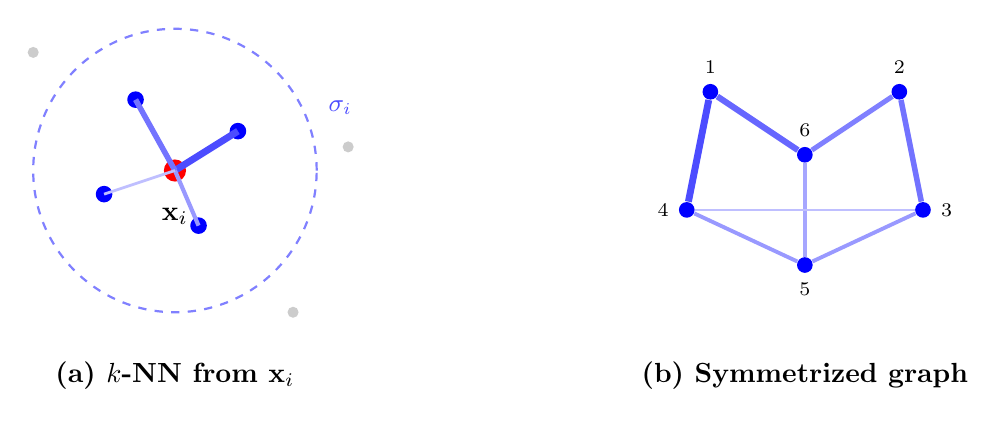
\begin{tikzpicture}[scale=1.0]
  % Left: k-NN graph construction
  \begin{scope}[shift={(-4,0)}]
    % Central point
    \fill[red] (0,0) circle (4pt);
    \node[below] at (0,-0.35) {$\mathbf{x}_i$};

    % Local neighborhood circle
    \draw[dashed, blue!50, thick] (0,0) circle (1.8);
    \node[blue!70] at (2.1,0.8) {\small $\sigma_i$};

    % Neighbors (k=4) with labels
    \fill[blue] (0.8,0.5) circle (3pt);
    \fill[blue] (-0.5,0.9) circle (3pt);
    \fill[blue] (0.3,-0.7) circle (3pt);
    \fill[blue] (-0.9,-0.3) circle (3pt);

    % Edges with varying thickness (weight)
    \draw[line width=2.5pt, blue!70] (0,0) -- (0.8,0.5);
    \draw[line width=2.0pt, blue!55] (0,0) -- (-0.5,0.9);
    \draw[line width=1.5pt, blue!40] (0,0) -- (0.3,-0.7);
    \draw[line width=1.0pt, blue!25] (0,0) -- (-0.9,-0.3);

    % Far points (not connected)
    \fill[gray!40] (2.2,0.3) circle (2pt);
    \fill[gray!40] (-1.8,1.5) circle (2pt);
    \fill[gray!40] (1.5,-1.8) circle (2pt);

    \node[font=\bfseries] at (0,-2.6) {(a) $k$-NN from $\mathbf{x}_i$};
  \end{scope}

  % Right: Symmetrized fuzzy graph
  \begin{scope}[shift={(4,0)}]
    % Points with labels
    \node[circle, fill=blue, inner sep=2pt, label=above:{\scriptsize $1$}] (n1) at (-1.2,1) {};
    \node[circle, fill=blue, inner sep=2pt, label=above:{\scriptsize $2$}] (n2) at (1.2,1) {};
    \node[circle, fill=blue, inner sep=2pt, label=right:{\scriptsize $3$}] (n3) at (1.5,-0.5) {};
    \node[circle, fill=blue, inner sep=2pt, label=left:{\scriptsize $4$}] (n4) at (-1.5,-0.5) {};
    \node[circle, fill=blue, inner sep=2pt, label=below:{\scriptsize $5$}] (n5) at (0,-1.2) {};
    \node[circle, fill=blue, inner sep=2pt, label=above:{\scriptsize $6$}] (n6) at (0,0.2) {};

    % Edges with varying line width (symmetric weights)
    \draw[line width=2.2pt, blue!60] (n1) -- (n6);
    \draw[line width=1.8pt, blue!50] (n2) -- (n6);
    \draw[line width=2.5pt, blue!70] (n1) -- (n4);
    \draw[line width=2.0pt, blue!55] (n2) -- (n3);
    \draw[line width=1.4pt, blue!40] (n4) -- (n5);
    \draw[line width=1.4pt, blue!40] (n3) -- (n5);
    \draw[line width=1.2pt, blue!35] (n6) -- (n5);
    \draw[line width=0.8pt, blue!25] (n4) -- (n3);

    \node[font=\bfseries] at (0,-2.6) {(b) Symmetrized graph};
  \end{scope}
\end{tikzpicture}
\caption{Construction of the fuzzy simplicial set. (a) For each point $\mathbf{x}_i$, edges connect to $k$ nearest neighbors with weights $w_{i \to j}$ that decay exponentially with distance (edge thickness indicates weight). The local scale $\sigma_i$ normalizes for varying density. (b) The final graph has symmetric weights obtained by fuzzy union: $w_{ij} = w_{i \to j} + w_{j \to i} - w_{i \to j} w_{j \to i}$.}
\label{fig:umap-graph}
\end{figure}

\subsection{The Optimization Problem}

Given the high-dimensional fuzzy graph $G^{(h)}$ with weights $\{w_{ij}^{(h)}\}$, UMAP seeks a low-dimensional embedding $\mathbf{y}_1, \dots, \mathbf{y}_N \in \mathbb{R}^m$ (typically $m = 2$ or $3$) whose fuzzy graph $G^{(\ell)}$ has similar structure.

\subsubsection{Low-Dimensional Edge Weights}

In the embedding space, edge weights are computed using a Student $t$-distribution kernel (similar to $t$-SNE):
\begin{equation}\label{eq:umap-low-weight}
  w_{ij}^{(\ell)} = \left(1 + a\|\mathbf{y}_i - \mathbf{y}_j\|^{2b}\right)^{-1},
\end{equation}
where $a, b > 0$ are hyperparameters (default: $a \approx 1.93$, $b \approx 0.79$, chosen to approximate a specific target distribution).

\begin{figure}[h]
\centering
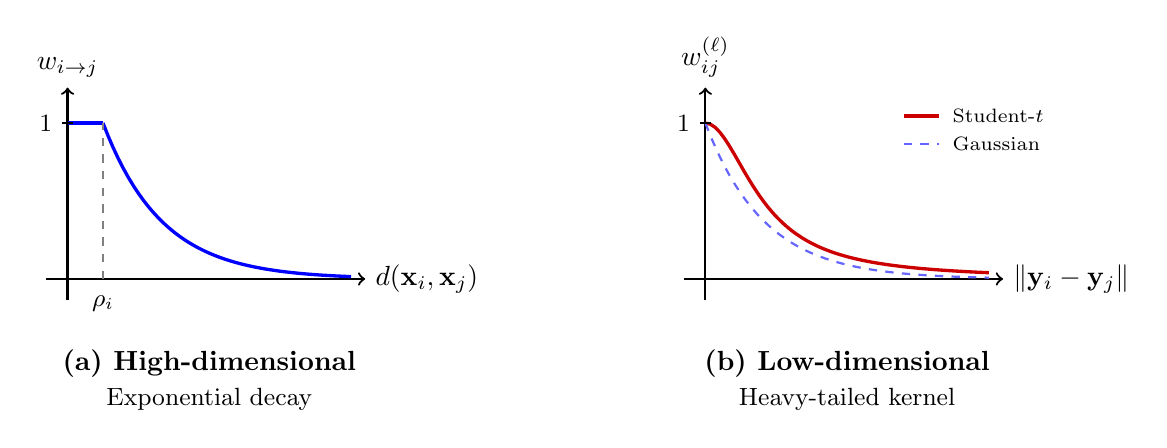
\begin{tikzpicture}[scale=0.9]
  % High-dimensional kernel
  \begin{scope}[shift={(-4.5,0)}]
    \draw[->, thick] (-0.3,0) -- (4.2,0) node[right] {$d(\mathbf{x}_i, \mathbf{x}_j)$};
    \draw[->, thick] (0,-0.3) -- (0,2.7) node[above] {$w_{i \to j}$};

    % Exponential decay starting from rho
    \draw[very thick, blue, domain=0.5:4, samples=50] plot (\x, {2.2*exp(-1.2*(\x-0.5))});
    \draw[very thick, blue] (0,2.2) -- (0.5,2.2);

    % Mark rho
    \draw[dashed, gray] (0.5,0) -- (0.5,2.2);
    \node[below] at (0.5,-0.1) {\small $\rho_i$};

    % Mark 1 on y-axis
    \draw (0.08,2.2) -- (-0.08,2.2) node[left] {\small $1$};

    \node[font=\bfseries] at (2,-1.2) {(a) High-dimensional};
    \node[font=\small] at (2,-1.7) {Exponential decay};
  \end{scope}

  % Low-dimensional kernel
  \begin{scope}[shift={(4.5,0)}]
    \draw[->, thick] (-0.3,0) -- (4.2,0) node[right] {$\|\mathbf{y}_i - \mathbf{y}_j\|$};
    \draw[->, thick] (0,-0.3) -- (0,2.7) node[above] {$w_{ij}^{(\ell)}$};

    % Student-t like (heavy tails) - red
    \draw[very thick, red!80!black, domain=0:4, samples=60] plot (\x, {2.2/(1+1.5*\x*\x)});

    % Gaussian for comparison (dashed blue)
    \draw[thick, dashed, blue!60, domain=0:4, samples=50] plot (\x, {2.2*exp(-1.2*\x)});

    % Mark 1 on y-axis
    \draw (0.08,2.2) -- (-0.08,2.2) node[left] {\small $1$};

    % Legend
    \draw[very thick, red!80!black] (2.8,2.3) -- (3.3,2.3);
    \node[right, font=\scriptsize] at (3.35,2.3) {Student-$t$};
    \draw[thick, dashed, blue!60] (2.8,1.9) -- (3.3,1.9);
    \node[right, font=\scriptsize] at (3.35,1.9) {Gaussian};

    \node[font=\bfseries] at (2,-1.2) {(b) Low-dimensional};
    \node[font=\small] at (2,-1.7) {Heavy-tailed kernel};
  \end{scope}
\end{tikzpicture}
\caption{Comparison of similarity kernels. (a) In high dimensions, edge weights decay exponentially from the nearest neighbor distance $\rho_i$. (b) In the embedding, UMAP uses a heavy-tailed Student-$t$ kernel (solid) instead of a Gaussian (dashed). The heavier tails allow moderately distant points to exert repulsive forces, preventing cluster collapse.}
\label{fig:umap-kernels}
\end{figure}

\subsubsection{Cross-Entropy Loss}

The discrepancy between the high-dimensional and low-dimensional fuzzy graphs is measured by fuzzy set cross-entropy:
\begin{equation}\label{eq:umap-loss}
  \mathcal{L}(\mathbf{y}_1, \dots, \mathbf{y}_N) = \sum_{i < j} \left[ w_{ij}^{(h)} \log\frac{w_{ij}^{(h)}}{w_{ij}^{(\ell)}} + (1 - w_{ij}^{(h)}) \log\frac{1 - w_{ij}^{(h)}}{1 - w_{ij}^{(\ell)}} \right].
\end{equation}

\begin{remark}[Interpretation of the loss]\leavevmode
  \begin{itemize}
    \item The first term penalizes when points that are close in high dimensions ($w_{ij}^{(h)}$ large) become far apart in the embedding ($w_{ij}^{(\ell)}$ small). This preserves \emph{local structure}.
    \item The second term penalizes when points that are far apart in high dimensions ($w_{ij}^{(h)}$ small) become close in the embedding ($w_{ij}^{(\ell)}$ large). This preserves \emph{global structure} and prevents collapse.
  \end{itemize}
\end{remark}

\begin{theorem}[UMAP gradient]\label{thm:umap-gradient}
  The gradient of the cross-entropy loss \eqref{eq:umap-loss} with respect to embedding point $\mathbf{y}_i$ is
  \begin{equation}\label{eq:umap-gradient}
    \frac{\partial \mathcal{L}}{\partial \mathbf{y}_i} = \sum_{j \neq i} \left[ \underbrace{-2ab \, w_{ij}^{(h)} \left(w_{ij}^{(\ell)}\right)^2 d_{ij}^{2(b-1)}}_{\text{attractive}}  + \underbrace{\frac{2ab \, (1-w_{ij}^{(h)}) w_{ij}^{(\ell)} d_{ij}^{2(b-1)}}{1 - w_{ij}^{(\ell)}}}_{\text{repulsive}} \right] (\mathbf{y}_i - \mathbf{y}_j),
  \end{equation}
  where $d_{ij} = \|\mathbf{y}_i - \mathbf{y}_j\|$ and $w_{ij}^{(\ell)} = (1 + a \, d_{ij}^{2b})^{-1}$.
\end{theorem}

\begin{proof}
  We compute the gradient in three steps.

  \textbf{Step 1: Derivative of the low-dimensional weight.}
  Let $d_{ij} = \|\mathbf{y}_i - \mathbf{y}_j\|$ denote the Euclidean distance. The low-dimensional weight is
  \[
    w_{ij}^{(\ell)} = \frac{1}{1 + a \, d_{ij}^{2b}}.
  \]
  Taking the derivative with respect to $d_{ij}^2$:
  \[
    \frac{\partial w_{ij}^{(\ell)}}{\partial (d_{ij}^2)} = \frac{-ab \, d_{ij}^{2(b-1)}}{(1 + a \, d_{ij}^{2b})^2} = -ab \, d_{ij}^{2(b-1)} \left(w_{ij}^{(\ell)}\right)^2.
  \]
  Since $d_{ij}^2 = \|\mathbf{y}_i - \mathbf{y}_j\|^2$, we have $\frac{\partial (d_{ij}^2)}{\partial \mathbf{y}_i} = 2(\mathbf{y}_i - \mathbf{y}_j)$. By the chain rule:
  \begin{equation}\label{eq:weight-gradient}
    \frac{\partial w_{ij}^{(\ell)}}{\partial \mathbf{y}_i} = -2ab \, d_{ij}^{2(b-1)} \left(w_{ij}^{(\ell)}\right)^2 (\mathbf{y}_i - \mathbf{y}_j).
  \end{equation}

  \textbf{Step 2: Derivative of the cross-entropy terms.}
  The loss decomposes as $\mathcal{L} = \sum_{i < j} \mathcal{L}_{ij}$ where
  \[
    \mathcal{L}_{ij} = w_{ij}^{(h)} \log\frac{w_{ij}^{(h)}}{w_{ij}^{(\ell)}} + (1 - w_{ij}^{(h)}) \log\frac{1 - w_{ij}^{(h)}}{1 - w_{ij}^{(\ell)}}.
  \]
  The high-dimensional weights $w_{ij}^{(h)}$ are constants (computed once from the input data). Differentiating with respect to $w_{ij}^{(\ell)}$:
  \[
    \frac{\partial \mathcal{L}_{ij}}{\partial w_{ij}^{(\ell)}} = \frac{-w_{ij}^{(h)}}{w_{ij}^{(\ell)}} + \frac{1 - w_{ij}^{(h)}}{1 - w_{ij}^{(\ell)}}.
  \]

  \textbf{Step 3: Combining via chain rule.}
  Applying the chain rule $\frac{\partial \mathcal{L}_{ij}}{\partial \mathbf{y}_i} = \frac{\partial \mathcal{L}_{ij}}{\partial w_{ij}^{(\ell)}} \cdot \frac{\partial w_{ij}^{(\ell)}}{\partial \mathbf{y}_i}$ and substituting \eqref{eq:weight-gradient}:
  \begin{align*}
    \frac{\partial \mathcal{L}_{ij}}{\partial \mathbf{y}_i}
     & = \left( \frac{-w_{ij}^{(h)}}{w_{ij}^{(\ell)}} + \frac{1 - w_{ij}^{(h)}}{1 - w_{ij}^{(\ell)}} \right) \cdot \left( -2ab \, d_{ij}^{2(b-1)} \left(w_{ij}^{(\ell)}\right)^2 (\mathbf{y}_i - \mathbf{y}_j) \right) \\
     & = 2ab \, d_{ij}^{2(b-1)} \left( w_{ij}^{(h)} \, w_{ij}^{(\ell)} - \frac{(1 - w_{ij}^{(h)}) \left(w_{ij}^{(\ell)}\right)^2}{1 - w_{ij}^{(\ell)}} \right) (\mathbf{y}_i - \mathbf{y}_j).
  \end{align*}
  Rearranging and summing over all $j \neq i$ (accounting for symmetry) yields \eqref{eq:umap-gradient}.
\end{proof}

\begin{corollary}[Attractive and repulsive forces]
  The gradient update $\mathbf{y}_i \leftarrow \mathbf{y}_i - \eta \frac{\partial \mathcal{L}}{\partial \mathbf{y}_i}$ decomposes into:
  \begin{itemize}
    \item \textbf{Attractive force} from neighbor $j$: When $w_{ij}^{(h)}$ is large (points are neighbors in high dimensions), the first term dominates, producing a force proportional to $-(\mathbf{y}_i - \mathbf{y}_j)$ that pulls $\mathbf{y}_i$ toward $\mathbf{y}_j$.
    \item \textbf{Repulsive force} from non-neighbor $k$: When $w_{ik}^{(h)}$ is small, the second term dominates, producing a force proportional to $+(\mathbf{y}_i - \mathbf{y}_k)$ that pushes $\mathbf{y}_i$ away from $\mathbf{y}_k$.
  \end{itemize}
\end{corollary}

\begin{remark}[Negative sampling]
  Computing the full gradient requires summing over all $O(N^2)$ pairs, which is prohibitive for large $N$. UMAP uses \emph{negative sampling}: for each edge $(i,j)$ with large $w_{ij}^{(h)}$, compute the attractive term exactly, but approximate the repulsive sum by sampling a small number of random ``negative'' points $k$ with probability proportional to their degree. This reduces complexity to $O(N)$ per iteration while preserving the gradient direction in expectation.
\end{remark}

\begin{figure}[h]
\centering
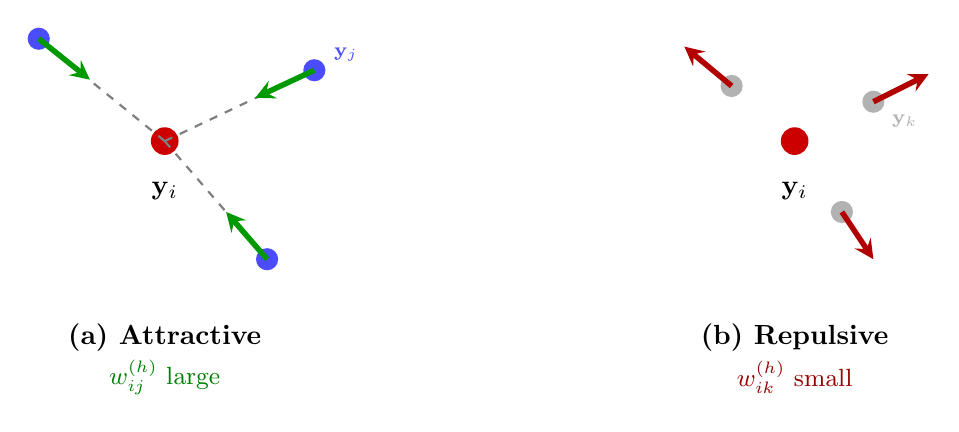
\begin{tikzpicture}[scale=1.0, >=stealth]
  % Attractive forces
  \begin{scope}[shift={(-4,0)}]
    % Central point
    \fill[red!80!black] (0,0) circle (5pt);
    \node[below] at (0,-0.4) {$\mathbf{y}_i$};

    % Neighbors being pulled (blue = high-dim neighbors)
    \fill[blue!70] (1.9,0.9) circle (4pt);
    \fill[blue!70] (-1.6,1.3) circle (4pt);
    \fill[blue!70] (1.3,-1.5) circle (4pt);

    % Dashed lines showing high-dim connection
    \draw[dashed, gray, thick] (0,0) -- (1.9,0.9);
    \draw[dashed, gray, thick] (0,0) -- (-1.6,1.3);
    \draw[dashed, gray, thick] (0,0) -- (1.3,-1.5);

    % Attractive arrows (pointing inward) - green
    \draw[->, line width=2pt, green!60!black] (1.9,0.9) -- (1.15,0.55);
    \draw[->, line width=2pt, green!60!black] (-1.6,1.3) -- (-0.95,0.78);
    \draw[->, line width=2pt, green!60!black] (1.3,-1.5) -- (0.78,-0.9);

    % Labels
    \node[blue!70, font=\scriptsize] at (2.3,1.1) {$\mathbf{y}_j$};
    \node[font=\bfseries] at (0,-2.5) {(a) Attractive};
    \node[font=\small, green!50!black] at (0,-3.0) {$w_{ij}^{(h)}$ large};
  \end{scope}

  % Repulsive forces
  \begin{scope}[shift={(4,0)}]
    % Central point
    \fill[red!80!black] (0,0) circle (5pt);
    \node[below] at (0,-0.4) {$\mathbf{y}_i$};

    % Non-neighbors (gray = not connected in high-dim)
    \fill[gray!60] (1.0,0.5) circle (4pt);
    \fill[gray!60] (-0.8,0.7) circle (4pt);
    \fill[gray!60] (0.6,-0.9) circle (4pt);

    % Repulsive arrows (pointing outward) - red
    \draw[->, line width=2pt, red!70!black] (1.0,0.5) -- (1.7,0.85);
    \draw[->, line width=2pt, red!70!black] (-0.8,0.7) -- (-1.4,1.2);
    \draw[->, line width=2pt, red!70!black] (0.6,-0.9) -- (1.0,-1.5);

    % Labels
    \node[gray!60, font=\scriptsize] at (1.4,0.25) {$\mathbf{y}_k$};
    \node[font=\bfseries] at (0,-2.5) {(b) Repulsive};
    \node[font=\small, red!60!black] at (0,-3.0) {$w_{ik}^{(h)}$ small};
  \end{scope}
\end{tikzpicture}
\caption{Forces during UMAP optimization. (a) Points that are neighbors in high dimensions (large $w_{ij}^{(h)}$, dashed lines) experience attractive forces pulling them together in the embedding. (b) Points that are distant in high dimensions (small $w_{ik}^{(h)}$, sampled as negative examples) experience repulsive forces pushing them apart. The balance preserves local structure while preventing global collapse.}
\label{fig:umap-forces}
\end{figure}

\begin{example}[Circle vs.\ Swiss roll: topology matters]\label{ex:circle-topology}
  A natural question arises: if UMAP ``unrolls'' the Swiss roll into a rectangle, would it unroll a \emph{circle} $S^1$ into a line segment?

  The answer is \textbf{no}. The key difference is \emph{topological}:
  \begin{itemize}
    \item The Swiss roll is homeomorphic to a rectangle $[0,1] \times [0,1]$---it has boundary and is \emph{simply connected} (any loop can be continuously shrunk to a point).
    \item The circle $S^1$ has no boundary and is \emph{not simply connected}---a loop around the circle cannot be shrunk to a point without leaving the manifold.
  \end{itemize}

  UMAP preserves local neighborhoods via the fuzzy simplicial set construction. For a circle, each point $\mathbf{x}_i$ has neighbors on both sides, forming a chain that wraps around:
  \[
    \mathbf{x}_1 \leftrightarrow \mathbf{x}_2 \leftrightarrow \cdots \leftrightarrow \mathbf{x}_N \leftrightarrow \mathbf{x}_1.
  \]
  To ``unroll'' this into a line segment $[a,b]$, UMAP would need to \emph{cut} the circle somewhere, separating two adjacent points $\mathbf{x}_i$ and $\mathbf{x}_{i+1}$ that have high edge weight $w_{i,i+1}^{(h)}$. This would incur a large attractive penalty in the cross-entropy loss \eqref{eq:umap-loss}.

  Instead, UMAP embeds the circle as a closed curve in $\mathbb{R}^2$---preserving both the local metric structure (nearby points stay nearby) and the global topology (the loop structure is maintained).
\end{example}

\begin{figure}[h]
\centering
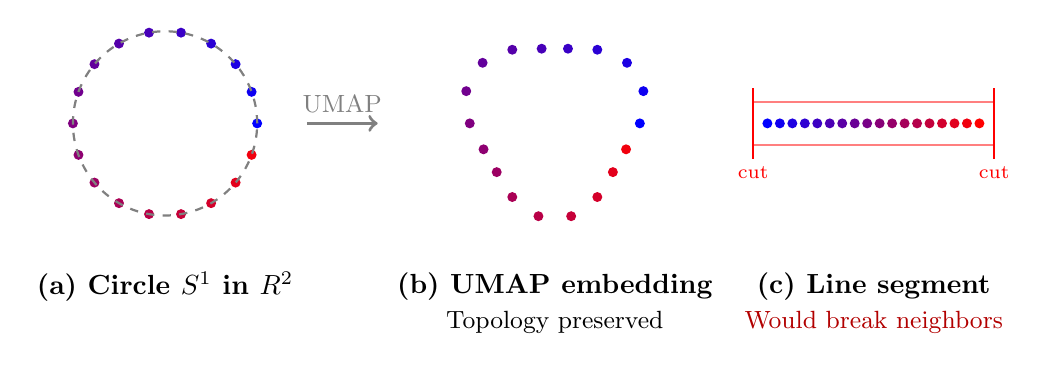
\begin{tikzpicture}[scale=0.9]
  % Left: Circle in high dimensions
  \begin{scope}[shift={(-4.5,0)}]
    % Draw circle with color gradient
    \foreach \angle in {0,20,...,340} {
      \pgfmathsetmacro{\col}{\angle/360*100}
      \fill[red!\col!blue] ({1.3*cos(\angle)}, {1.3*sin(\angle)}) circle (2pt);
    }
    \draw[gray, thick, dashed] (0,0) circle (1.3);
    \node[font=\bfseries] at (0,-2.3) {(a) Circle $S^1$ in $\mathbb{R}^2$};
  \end{scope}

  % Arrow
  \draw[->, very thick, gray] (-2.5,0) -- (-1.5,0) node[midway, above] {\small UMAP};

  % Right: Circle preserved (not unrolled)
  \begin{scope}[shift={(1,0)}]
    % Draw slightly deformed circle (UMAP output)
    \foreach \angle in {0,20,...,340} {
      \pgfmathsetmacro{\col}{\angle/360*100}
      \pgfmathsetmacro{\r}{1.2 + 0.15*sin(3*\angle)}
      \fill[red!\col!blue] ({\r*cos(\angle)}, {\r*sin(\angle)}) circle (2pt);
    }
    \node[font=\bfseries] at (0,-2.3) {(b) UMAP embedding};
    \node[font=\small] at (0,-2.8) {Topology preserved};
  \end{scope}

  % Wrong: if it were unrolled
  \begin{scope}[shift={(5.5,0)}]
    % Line segment (wrong!)
    \foreach \i in {0,1,...,17} {
      \pgfmathsetmacro{\col}{\i/17*100}
      \fill[red!\col!blue] ({-1.5 + \i*0.176}, 0) circle (2pt);
    }
    \draw[thick, red, opacity=0.5] (-1.7,-0.3) -- (1.7,-0.3) -- (1.7,0.3) -- (-1.7,0.3) -- cycle;
    \draw[red, thick] (-1.7,-0.5) -- (-1.7,0.5);
    \draw[red, thick] (1.7,-0.5) -- (1.7,0.5);
    \node[red, font=\scriptsize] at (-1.7, -0.7) {cut};
    \node[red, font=\scriptsize] at (1.7, -0.7) {cut};
    \node[font=\bfseries] at (0,-2.3) {(c) Line segment};
    \node[font=\small, red!70!black] at (0,-2.8) {Would break neighbors};
  \end{scope}
\end{tikzpicture}
\caption{UMAP preserves topology. (a) Points sampled uniformly from a circle, colored by angle. (b) UMAP embeds this as a closed curve, preserving the cyclic neighbor structure. (c) Unrolling to a line segment would require cutting the circle, separating neighbors that have high affinity $w_{ij}^{(h)}$---UMAP's loss function penalizes this.}
\label{fig:circle-topology}
\end{figure}

\subsection{Algorithm Summary}

\begin{enumerate}
  \item \textbf{Construct $k$-NN graph}: For each $\mathbf{x}_i$, find its $k$ nearest neighbors.
  \item \textbf{Compute local scales}: Solve \eqref{eq:umap-sigma} for each $\sigma_i$ using binary search.
  \item \textbf{Build fuzzy graph}: Compute directed weights \eqref{eq:umap-weight} and symmetrize via \eqref{eq:umap-symmetrize}.
  \item \textbf{Initialize embedding}: Use spectral embedding (eigenvectors of graph Laplacian) or random initialization.
  \item \textbf{Optimize}: Minimize cross-entropy \eqref{eq:umap-loss} via SGD with negative sampling.
\end{enumerate}

\subsection{Comparison with PCA}

\begin{center}
  \begin{tabular}{lll}
    \hline
    \textbf{Property}        & \textbf{PCA}          & \textbf{UMAP}                    \\
    \hline
    Structure captured       & Linear (subspaces)    & Nonlinear (manifolds)            \\
    Objective                & Maximize variance     & Preserve fuzzy topology          \\
    Computational complexity & $O(d^2 N + d^3)$      & $O(N^{1.14})$ empirically        \\
    Deterministic            & Yes                   & No (stochastic optimization)     \\
    Out-of-sample extension  & Simple ($\mathbf{W}^{\mathsf{T}}\mathbf{x}$) & Requires approximation \\
    Interpretability         & Principal components  & Less interpretable               \\
    \hline
  \end{tabular}
\end{center}

\subsection{Applications}

\subsubsection{Single-Cell RNA Sequencing}
In computational biology, single-cell RNA-seq produces expression profiles for thousands of genes across thousands of cells. UMAP is the standard tool for visualizing this data, revealing cell types, developmental trajectories, and rare cell populations that PCA would fail to separate.

\subsubsection{Natural Language Processing}
Word embeddings (e.g., Word2Vec, GloVe) live in high-dimensional spaces where semantic relationships are encoded as directions. UMAP can project these to 2D for visualization, revealing clusters of semantically related words while preserving analogical structure.

\subsubsection{Image Embeddings}
Deep neural networks produce high-dimensional feature vectors for images. UMAP visualization of these embeddings reveals how the network organizes visual concepts, useful for debugging classifiers and understanding learned representations.

\subsubsection{Text Embeddings on the Unit Sphere}

Modern text embedding models (OpenAI's \texttt{text-embedding-ada-002}, Cohere, Voyage, etc.) produce high-dimensional vectors $\mathbf{v} \in \mathbb{R}^d$ (typically $d = 1536$ or $d = 3072$) that are $L^2$-normalized to lie on the unit sphere:
\[
  \|\mathbf{v}\| = 1, \quad \text{so } \mathbf{v} \in S^{d-1}.
\]
For these embeddings, similarity is measured by \emph{cosine similarity}, which on the unit sphere equals the dot product: $\cos\theta = \mathbf{v}_i^\top \mathbf{v}_j$.

\begin{remark}[Practical considerations for UMAP on text embeddings]\label{rem:umap-text-embeddings}\leavevmode
  \begin{enumerate}
    \item \textbf{Use cosine or angular distance}: Since the embeddings lie on $S^{d-1}$, Euclidean distance in $\mathbb{R}^d$ is a monotonic transformation of cosine similarity:
    \[
      \|\mathbf{v}_i - \mathbf{v}_j\|^2 = 2(1 - \mathbf{v}_i^\top \mathbf{v}_j) = 2(1 - \cos\theta_{ij}).
    \]
    UMAP with \texttt{metric='cosine'} or \texttt{metric='euclidean'} will produce similar results on normalized vectors, but cosine is semantically clearer.

    \item \textbf{Beware of density distortion}: Text corpora are fundamentally non-uniform---common topics (sports, politics) have dense clusters while niche topics (15th-century Flemish art) are sparse. Per Remark~\ref{rem:umap-sphere}:
    \begin{itemize}
      \item Cluster \emph{sizes} in the UMAP plot do not reflect true cluster sizes in the corpus.
      \item A cluster of 10,000 news articles about politics may appear similar in size to 100 articles about a rare disease.
      \item Inter-cluster distances are unreliable for comparing semantic similarity across density regimes.
    \end{itemize}

    \item \textbf{What UMAP \emph{does} preserve}: Despite density distortion, UMAP reliably preserves:
    \begin{itemize}
      \item \emph{Neighborhood membership}: Documents that are semantically similar will be placed near each other.
      \item \emph{Cluster separation}: Distinct topics will form visually separate clusters.
      \item \emph{Relative structure within density-homogeneous regions}: Within a single cluster, local structure is meaningful.
    \end{itemize}

    \item \textbf{Recommended workflow}:
    \begin{itemize}
      \item Use UMAP for \emph{exploration}: identifying clusters, finding outliers, understanding corpus structure.
      \item For \emph{quantitative analysis} (e.g., ``how similar are these two documents?''), use cosine similarity directly in the original $\mathbb{R}^d$ space.
      \item To compare cluster sizes or densities, compute statistics in the original space, not from the UMAP coordinates.
      \item Consider coloring points by metadata (date, source, label) to interpret clusters, since position alone can be misleading.
    \end{itemize}

    \item \textbf{Hyperparameter guidance}:
    \begin{itemize}
      \item \texttt{n\_neighbors}: Larger values (e.g., 30--50) preserve more global structure; smaller values (e.g., 5--15) emphasize local clusters. For text embeddings with many fine-grained topics, start with 15.
      \item \texttt{min\_dist}: Controls how tightly points cluster. For visualization, 0.1 works well; for preserving more structure, try 0.0.
      \item \texttt{n\_components}: Usually 2 for visualization; 3 for interactive 3D plots.
    \end{itemize}
  \end{enumerate}
\end{remark}

